\documentclass[11pt,a4paper]{article}
% Shared macros for the Crossfade LaTeX documents.
\usepackage[T1]{fontenc}
\usepackage[utf8]{inputenc}
\usepackage{lmodern}
\usepackage{microtype}
\usepackage{amsmath,amssymb,amsthm,mathtools}
\usepackage{bm}
\usepackage{booktabs,array,longtable}
\usepackage{enumitem}
\usepackage{geometry}
\geometry{a4paper,margin=25mm}
\usepackage{xcolor}
\usepackage[hidelinks]{hyperref}
\usepackage[numbers,sort&compress]{natbib}
\usepackage{caption}
\captionsetup{font=small,labelfont=bf}
\usepackage{multirow}

\theoremstyle{plain}
\newtheorem{proposition}{Proposition}[section]
\newtheorem{lemma}[proposition]{Lemma}
\newtheorem{corollary}[proposition]{Corollary}
\theoremstyle{definition}
\newtheorem{definition}[proposition]{Definition}
\newtheorem{assumption}[proposition]{Assumption}
\newtheorem{hypothesis}[proposition]{Hypothesis}
\theoremstyle{remark}
\newtheorem{remark}[proposition]{Remark}
\newtheorem{question}{Check}

\DeclareMathOperator{\E}{\mathbb{E}}
\DeclareMathOperator{\sinc}{sinc}
\DeclareMathOperator{\sgn}{sgn}
\DeclareMathOperator{\supp}{supp}
\DeclareMathOperator{\dist}{dist}
\DeclareMathOperator{\Var}{Var}
\newcommand{\R}{\mathbb{R}}
\newcommand{\C}{\mathbb{C}}
\newcommand{\Z}{\mathbb{Z}}
\newcommand{\dd}{\,\mathrm{d}}
\newcommand{\jj}{\mathrm{j}}
\newcommand{\ee}{\mathrm{e}}
\newcommand{\SH}{S_{\mathrm{H}}}
\newcommand{\CH}{C_{\mathrm{H}}}
\newcommand{\hW}{h_{\mathrm{W}}}
\newcommand{\Pit}{\Pi_{\tau}}
\newcommand{\Pin}{\Pi_{\nu}}
\newcommand{\PiL}{\Pi_{L}}
\newcommand{\Pif}{\Pi_{f}}
\newcommand{\Pih}{\Pi_{h}}
\newcommand{\Pis}{\Pi_{s}}
\newcommand{\betaB}{\beta_{B}}
\newcommand{\tagG}{\textbf{[G]}}
\newcommand{\tagP}{\textbf{[P]}}
\newcommand{\tagH}{\textbf{[H]}}
\newcommand{\code}[1]{\texttt{#1}}
\newcommand{\rms}{\sigma_{\tau}}
\newcommand{\dspread}{\sigma_{\nu}}
\newcommand{\Narr}{N_{\mathrm{arr}}}
\newcommand{\cbot}{c_{b}}
\newcommand{\rhob}{\rho_{b}}
\newcommand{\cw}{c}
\newcommand{\rhow}{\rho}
\setlist{nosep}

\setlength{\tabcolsep}{4pt}
\usepackage{titlesec}
\usepackage{tikz}\usetikzlibrary{arrows.meta,positioning,shapes.geometric,calc}
\usepackage{graphicx}
\titleformat{\part}[display]{\normalfont\Large\bfseries\filcenter}{Part \thepart}{6pt}{\huge}
\titlespacing*{\part}{0pt}{24pt}{18pt}

\title{Crossfade\\[4pt]\large A capability-aware evidence and experiment platform for wave-propagation inference\\[2pt]\normalsize Full thesis, specification v0.3 and build pack v0.3, in one document}
\author{Jason}
\date{2026-09-21}

\begin{document}
\maketitle

\begin{abstract}
\noindent Crossfade connects sonar, HF skywave radar and RF systems through a common channel vocabulary anchored on the channel spreading function, and it measures where learned structure transfers between domains instead of assuming it. This document is the complete thesis: the motivation and the three separable contracts the platform commits to; the physics and mathematics it relies on, with the regime coordinates that turn ``does it transfer?'' into a preregisterable hypothesis; the identifiability limits that no estimator removes; the architecture, the five record types and the twenty-five invariants that make every result auditable; the models, the training objective and the baseline ladder; the typed treatment of uncertainty; the evaluation protocol with its three gates; the build plan in four slices with their acceptance criteria; the decision register; and the open questions for the sonar lead, two of which are on the critical path. Every requirement is tagged as an engineering guarantee \tagG{}, a provisional choice \tagP{}, or a hypothesis \tagH{}, and the tag decides what happens when it fails: a bug is fixed, a component is swapped, or a result is recorded.
\end{abstract}

\tableofcontents
\clearpage

% =====================================================================
\part{Motivation and claims}

\section{What Crossfade is}

The idea came from a conversation between a sonar and cross-domain signals lead and an ML lead. Every display anyone looks at, a range--Doppler map, a beam-level spectrogram, a cepstrum, is a measurement of the propagation channel's response, and the time-varying impulse response or the scattering function is what actually carries the answer: whether a target is there, whether it is closing, what the environment is doing. If you can estimate it, in the sonar lead's words, you have won. The same object describes an ocean waveguide, the Earth--ionosphere duct and an urban RF channel; the ionosphere is ``the ocean flipped upside down''. The question that followed was whether a model could learn what those channels have in common so that each new domain, environment or system needs less bespoke data and modelling, and where the modern tools, self-supervised encoders, physics-informed networks, large language models, actually fit.

Crossfade is the version of that idea that survived two rounds of review. The channel is still the centre. What changed is that we now know which parts of the idea the physics supports, which parts are hypotheses to measure, and where the machine learning and the language model sit so that they cannot quietly take over the science.

\paragraph{The one-sentence design.} Every quantity the platform estimates is defined as a functional of a named channel representation; every record carries units, coordinates, capabilities, processing history and lineage; every run has typed result states that are never filled with a passing value by default; every claim of transfer resolves to a preregistered comparison at a declared physical regime; and the language model reads records and writes drafts but never a number.

\section{Three separable contracts}

Crossfade commits to three contracts, and the platform stays useful if only the first holds.

\begin{center}\small
\begin{tabular}{@{}p{3.2cm}p{5.6cm}p{6cm}@{}}
\toprule
Contract & Claim & Evidence that it holds \\
\midrule
Interoperability & Any wave-sensing system's outputs can be ingested with units, coordinates, processing history and capability description intact, and replayed & A new domain connects through a domain pack without changing the core; a result reproduces from archived evidence \\
Representation transfer & A shared encoder pretrained on one domain reduces the target-domain data needed to estimate a declared quantity & Frozen-encoder few-shot gain over from-scratch at declared budgets, with effect size and uncertainty \\
Evidence fusion & Multiple results about one situation combine under a declared dependence model & Duplicate evidence is never double-counted; unknown dependence withholds numerical fusion \\
\bottomrule
\end{tabular}
\end{center}

\section{Three kinds of statement}

\begin{center}\small
\begin{tabular}{@{}p{2.6cm}p{7cm}p{5cm}@{}}
\toprule
Tag & Meaning & On failure \\
\midrule
\tagG{} Guarantee & A property the software enforces: immutability, provenance, typed states, leakage checks, reproducible comparison & Bug; fix the software; a test exists or must be written \\
\tagP{} Provisional & An architectural choice made now and replaceable later: canonical anchor kind, encoder family, storage backend & Swap the component; contracts unchanged \\
\tagH{} Hypothesis & A scientific claim to be measured: transfer at matched regime, usefulness of a regime coordinate, benefit of routing & Record the result in the atlas; the platform is unaffected \\
\bottomrule
\end{tabular}
\end{center}

\section{What Crossfade is not}

\begin{itemize}
\item Not a universal physics-informed neural network. PDE-residual PINNs fail at high wavenumber through spectral bias \citep{krishnapriyan2021}, which is exactly the regime of wave propagation. Physics enters as structural priors on the channel and as forward models in domain packs, where available.
\item Not an LLM that reads latent vectors. The LLM sits on typed records, explains, retrieves, and drafts pack metadata for human approval.
\item Not a replacement for existing processing chains. Legacy systems connect through output-only packs and are never written to.
\item Not a single latent space, and not a required reconstruction of one universal object from every input. Sharing is partial, per descriptor, and earned by benchmark.
\end{itemize}

Two tensions in the original conversation are resolved as follows. First, ``factor out the channel'' versus ``the channel is the information'': a variable is a nuisance relative to a task, never inherently, so each task specification says what is retained, conditioned on, or marginalized. Second, ``domain-invariant'' versus ``no information loss'': these cannot both hold in one compressed representation, so the archive preserves the source evidence, each derived representation declares what it retains, and private pathways carry what the shared one drops.

\section{How the thesis was formed}
\label{sec:provenance}

The record of how we got here is kept in the repository's \code{archive/} directory. In order:
\begin{enumerate}
\item \textbf{The transcript.} The sonar lead's claims: the channel as the common thread; cepstral and blind channel-estimation work; the overlapped-source problem where many signals share one band and multipath traces cannot be assigned to sources; the practical question of window and FFT lengths across domains; the desire for a training objective that aligns the spaces ``naturally without carving something up''.
\item \textbf{Two plans.} A first-principles plan that wrote down the generative structure $y_d=\mathcal M_d[\mathcal F_d(\theta;c_d)]+\varepsilon_d$ and derived the architecture from it, and a physics-modelling plan that supplied the representation atlas, the capability registry, the evidence graph and a workbench that stays useful when every transfer hypothesis fails.
\item \textbf{The synthesis.} A referee document found the plans agree on roughly eighty percent of their content and are complementary where they differ, and added three things neither said: name the anchor as the spreading function; make the regime a dimensionless coordinate; take self-supervised pretraining on paired views seriously.
\item \textbf{Spec v0.1 and an external architecture review.} The review's facts were examined claim by claim and found correct; its scaffolding was about twice the needed size (thirteen record types, twelve slices, a \code{conditional} assessment state with an authorization step). Its contract amendments were adopted with three modifications; its scaffolding was collapsed.
\item \textbf{Spec v0.2, the build-pack assessment, and v0.3.} The v0.2 build pack was dissected against one question: is this the simplest way to achieve the same result? The answer produced build pack v0.3, one Python package with five modules, and spec v0.3 aligned to it.
\item \textbf{The W0 workbench.} The first slice was implemented test-first on a branch and is waiting on the sonar lead's review before merging.
\end{enumerate}

\paragraph{Corrections we made to our own earlier claims.} These are worth listing because the reviewer for whom this document is written would have caught each of them.
\begin{itemize}
\item v0.1 called delay--Doppler ``the'' narrowband form and delay--scale ``the'' wideband form. Both always exist; what changes with $TB\,(v/c)$ is sparsity (Proposition~\ref{prop:rangewalk}).
\item v0.1 called resampling, windowing and carrier retune ``conventions''. They are lossy processing or physical intervention, and each transform is now classified and tested individually.
\item v0.1 claimed that contrasting a waveform with its own spectrogram and its own estimated CIR makes shared content identifiable. A deterministic re-representation has no nuisance to strip; only views with independent nuisance variation do (Section~\ref{sec:ident}).
\item v0.1's placeholder regime ranges were disjoint in $M$ and $\betaB$ while the pilot required overlap. Resolved as per-descriptor matching, which produced the overlap result (Proposition~\ref{prop:overlap}).
\item Citation corrections found while checking sources against the record: the bilinear-model paper is by Tian, Lee, Romberg, Durofchalk and Sabra (2020), not Sabra and Dowling; the ray-based blind deconvolution paper is Sabra, Song and Dowling (2010); Altes' wideband ambiguity paper is 1973; the 2011 time-scale characterization paper is by Chude-Okonkwo, Ngah and Abd Rahman; the CSI-CLIP++ authors are Jiang, Yu, Li, Gao and Xu.
\end{itemize}

% =====================================================================
\part{Physics and mathematics}
% math-core.tex — the mathematics of Crossfade. Included by both
% crossfade-math.tex and crossfade-full.tex. Section numbering comes from
% the including document.

\section{Notation and conventions}
\label{sec:notation}

\begin{center}
\small
\begin{tabular}{@{}lll@{}}
\toprule
Symbol & Meaning & Units \\
\midrule
$x(t),\,y(t)$ & transmitted and received signal (complex baseband unless stated) & -- \\
$s(t)$ & source waveform; $s_a(t)$ its analytic signal & -- \\
$h(t,\tau)$ & time-varying impulse response (Bello) & s$^{-1}$ \\
$\SH(\tau,\nu)$ & delay--Doppler spreading function & -- \\
$\hW(\tau,\alpha)$ & delay--scale spreading function & -- \\
$\CH(\tau,\nu)$ & scattering function, $\E|\SH|^2$ under WSSUS & -- \\
$P(\tau)$ & power--delay profile (PDP) & -- \\
$f_c,\,B,\,T$ & carrier, bandwidth, observation length & Hz, Hz, s \\
$c$ & propagation speed in the medium & m/s \\
$v$ & radial relative speed, positive when closing & m/s \\
$M=v/c$ & Mach number & 1 \\
$\betaB=B/f_c$ & fractional bandwidth & 1 \\
$\rms,\,\dspread$ & RMS delay spread, RMS Doppler spread & s, Hz \\
$\Pit,\Pin,\PiL,\Pif,\Pih,\Pis$ & regime groups, Section~\ref{sec:regime} & 1 \\
$\{(\tau_k,a_k)\}_{k=1}^{K}$ & arrival list: delays and complex gains & s, 1 \\
$D,\,z_s,\,z_r,\,r$ & water depth, source depth, receiver depth, range & m \\
$\cbot,\rhob$ & bottom half-space sound speed and density & m/s, kg/m$^3$ \\
\bottomrule
\end{tabular}
\end{center}

Fourier transform convention: $X(f)=\int x(t)\,\ee^{-\jj 2\pi f t}\dd t$. Scale $\alpha>1$ means time compression (a closing source). Every equation is tagged: \tagG{} for something the software enforces, \tagP{} for a convention or modelling choice that can be swapped without changing a contract, \tagH{} for a scientific claim the benchmark measures. Items marked \emph{Check} are the ones we most want the reader to confirm, correct, or replace.

% ---------------------------------------------------------------------------
\section{The channel and its representations}
\label{sec:channel}

\subsection{Linear time-varying channel}

A single-input single-output propagation channel is modelled as a linear time-varying (LTV) operator $\mathcal H$ with kernel $h(t,\tau)$ \citep{bello1963}:
\begin{equation}
  y(t) = (\mathcal H x)(t) = \int h(t,\tau)\, x(t-\tau)\dd\tau .
  \label{eq:ltv}
\end{equation}
$h(t,\tau)$ is the response at time $t$ to an impulse launched at time $t-\tau$. Its Fourier transform in $t$ is the \emph{delay--Doppler spreading function},
\begin{equation}
  \SH(\tau,\nu) = \int h(t,\tau)\,\ee^{-\jj 2\pi \nu t}\dd t,
  \qquad
  y(t) = \iint \SH(\tau,\nu)\, x(t-\tau)\,\ee^{\jj 2\pi\nu t}\dd\tau\dd\nu ,
  \label{eq:dd}
\end{equation}
so the channel is a superposition of delay-and-frequency-shift operators. The other two Bello functions follow by Fourier transform in $\tau$: the time-varying transfer function $L_{\mathrm H}(t,f)=\int h(t,\tau)\ee^{-\jj 2\pi f\tau}\dd\tau$ and the Doppler-variant transfer function.

\begin{proposition}[Existence]
\label{prop:existence}
Equation~\eqref{eq:dd} holds for any LTV operator whose kernel $h(t,\tau)$ is a tempered distribution in $t$; the delay--Doppler representation is not a narrowband approximation but a change of coordinates on the kernel \citep{matz2013}.
\end{proposition}
\noindent This is the correction made to v0.1 of the spec, which had called delay--Doppler ``the narrowband form''. What depends on the regime is not existence but \emph{sparsity} (Proposition~\ref{prop:rangewalk}).

\subsection[Delay--scale (wideband) representation]{Delay--scale (wideband) representation\hfill{\normalfont\small \tagP{}}}

The same operator can be written as a superposition of delay-and-scale operators,
\begin{equation}
  y(t) = \iint \hW(\tau,\alpha)\,\sqrt{\alpha}\; x\big(\alpha (t-\tau)\big)\dd\tau\dd\alpha ,
  \qquad \alpha>0,
  \label{eq:ds}
\end{equation}
where $\hW$ is the delay--scale (wideband) spreading function \citep{altes1973,chude2011}. A single reflector with radial closing speed $v$ produces, in passband,
\begin{equation}
  \alpha = \frac{c+v}{c-v}\approx 1+\frac{2v}{c} \ \text{(monostatic, two-way)},\qquad
  \alpha = 1+\frac{v}{c} \ \text{(one-way, passive)} .
  \label{eq:alpha}
\end{equation}
Two conventions are pack-declared and recorded in the anchor's \code{normalization} field rather than fixed by the core: the $\sqrt{\alpha}$ energy normalization, and whether the scaling is written $x(\alpha(t-\tau))$ as above or $x(\alpha t-\tau)$, which differ by $\tau\mapsto\alpha\tau$.

\subsection{When is one representation sparse? The range-walk number}

Consider one path with delay $\tau_0$ and scale $\alpha_0$, observed over $t\in[0,T]$, acting on a passband signal $x(t)=u(t)\ee^{\jj2\pi f_c t}$ with envelope bandwidth $B$. In baseband the path is the operator
\begin{equation}
  u \mapsto \sqrt{\alpha_0}\;u\big(\alpha_0(t-\tau_0)\big)\,\ee^{\jj 2\pi \nu_0 t}\,\ee^{-\jj 2\pi f_c\alpha_0\tau_0},
  \qquad \nu_0 = (\alpha_0-1) f_c ,
  \label{eq:pathop}
\end{equation}
whose Bello kernel is $h(t,\tau)=\sqrt{\alpha_0}\,\ee^{\jj2\pi\nu_0 t}\ee^{-\jj2\pi f_c\alpha_0\tau_0}\,\delta\big(\tau-\tau(t)\big)$ with the \emph{drifting delay}
\begin{equation}
  \tau(t) = \alpha_0\tau_0 + (1-\alpha_0)\,t .
  \label{eq:drift}
\end{equation}

\begin{proposition}[Range walk]
\label{prop:rangewalk}
Let $g$ be the delay-resolution kernel of the waveform (width $1/B$) and $\tilde h = h *_\tau g$ the resolution-limited kernel. Over an observation of length $T$, the resolution-limited spreading function $\tilde S_{\mathrm H}(\tau,\nu)$ of the single path~\eqref{eq:pathop} has support of extent
\begin{equation}
  \Delta\tau \approx \max\!\Big(\tfrac{1}{B},\,|\alpha_0-1|\,T\Big),
  \qquad
  \Delta\nu \approx \max\!\Big(\tfrac{1}{T},\,|\alpha_0-1|\,B\Big),
\end{equation}
that is, about $\max(1,\Pis)$ resolution cells along each axis, where
\begin{equation}
  \boxed{\;\Pis \;=\; T\,B\,|\alpha_0-1| \;=\; T B\,M \ \ \text{(one-way)}\;}
  \label{eq:Pis}
\end{equation}
is the range-walk number. In the delay--scale plane the same path is a single point $(\tau_0,\alpha_0)$ at the resolution of the wideband ambiguity function.
\end{proposition}

\begin{proof}[Sketch]
Write $\tilde h(t,\tau)=\sqrt{\alpha_0}\,\ee^{\jj2\pi\nu_0 t}\,g\big(\tau-\tau(t)\big)$ up to a constant phase. Substituting $s=\tau-\tau(t)$ in the Fourier integral over $t\in[0,T]$,
\[
  \tilde S_{\mathrm H}(\tau,\nu)
  = \frac{\sqrt{\alpha_0}}{\alpha_0-1}\,\ee^{-\jj 2\pi(\nu-\nu_0)\,t^\ast(\tau)}\;
    G\!\left(\frac{\nu-\nu_0}{\alpha_0-1}\right)\!\Big|_{s\in\text{window}},
  \qquad t^\ast(\tau)=\frac{\tau-\alpha_0\tau_0}{1-\alpha_0},
\]
where $G$ is the transform of $g$ and has width $B$. The delay support is the set of $\tau$ for which $t^\ast(\tau)\in[0,T]$, of length $|\alpha_0-1|T$; the Doppler support is where $G$ is non-negligible, of width $|\alpha_0-1|B$. When either is below one resolution cell the window and kernel widths take over.
\end{proof}

\begin{remark}
Equation~\eqref{eq:Pis} is the Kelly--Wishner narrowband condition $TB\,(2v/c)\ll1$ for the monostatic case \citep{kelly1965}, written as a dimensionless group. In the regime coordinates of Section~\ref{sec:regime}, $\Pis = M\cdot TB = M\,\betaB\,(f_cT)$. It is a property of the waveform and the motion jointly, so the threshold $\theta$ at which a pack switches canonical kind from \code{delay\_doppler} to \code{delay\_scale} is declared and tested by the pack, per regime box, and is not core logic.
\end{remark}

\begin{question}
Is $\Pis=TB|\alpha-1|$ the quantity you would use to decide between delay--Doppler and delay--scale processing, and is a threshold of order one (we have used $\theta\approx0.1$ as a placeholder) the right order? For the passive wideband sonar case, is there structure in the modal picture that the delay--scale form loses at ranges you care about?
\end{question}

\subsection[Realization versus statistic]{Realization versus statistic\hfill{\normalfont\small \tagG{} for the field, \tagP{} for WSSUS}}

$\SH$ describes one channel realization. If the channel is wide-sense stationary in $t$ with uncorrelated scattering in $\tau$ (WSSUS), then
\begin{equation}
  \E\big[\SH(\tau,\nu)\,\SH^\ast(\tau',\nu')\big] = \CH(\tau,\nu)\,\delta(\tau-\tau')\,\delta(\nu-\nu'),
  \label{eq:wssus}
\end{equation}
and $\CH$ is the \emph{scattering function}. Its marginals are the power--delay profile and the Doppler power profile,
\begin{equation}
  P(\tau)=\int \CH(\tau,\nu)\dd\nu, \qquad P_\nu(\nu)=\int \CH(\tau,\nu)\dd\tau .
  \label{eq:pdp}
\end{equation}
For a single realization the time-averaged delay profile is $\hat P_T(\tau)=\frac1T\int_0^T|h(t,\tau)|^2\dd t$, which converges to $P$ under WSSUS and ergodicity. The wideband analogue replaces $(\tau,\nu)$ with $(\tau,\alpha)$ \citep{chude2011}. Every anchor record states which of these it holds through \code{statistical\_semantics} $\in\{$\code{realization}, \code{expectation}, \code{estimate}, \code{posterior\_samples}, \code{pseudo\_label}$\}$, and WSSUS, when an operation needs it, is a declared parameter \code{assume\_wssus}, never a default.

\begin{question}
Are there operational cases where you would want a \emph{local} scattering function (non-WSSUS, per \citealp{matz2011}) as a first-class kind, rather than a realization plus a time-series of PDPs?
\end{question}

% ---------------------------------------------------------------------------
\section{Descriptors as functionals of a named representation}
\label{sec:descriptors}

The anchor is a vocabulary, not a required payload: every quantity Crossfade estimates is defined as a functional of a \emph{named} channel representation. In the contracts this is one string per quantity, \code{canonical\_kind}, taking one of the values \code{impulse\_response}, \code{delay\_doppler}, \code{delay\_scale}, \code{power\_statistic} or \code{descriptors\_only}, or else the tag \code{not\_channel}. \tagG{} that the string exists; \tagP{} the list.

\subsection{Moments of the power--delay profile}

\begin{definition}[Delay moments]
For a non-negative profile $P$ with $0<\int P<\infty$,
\begin{equation}
  \bar\tau = \frac{\int \tau P(\tau)\dd\tau}{\int P(\tau)\dd\tau},\qquad
  \rms^2 = \frac{\int (\tau-\bar\tau)^2 P(\tau)\dd\tau}{\int P(\tau)\dd\tau}.
  \label{eq:moments}
\end{equation}
For a discrete profile $\{(\tau_k, E_k)\}$ with weights $w_k=E_k/\sum_j E_j$: $\bar\tau=\sum_k w_k\tau_k$, $\rms^2=\sum_k w_k(\tau_k-\bar\tau)^2$.
\end{definition}
The Doppler spread $\dspread$ is the same functional of $P_\nu$. Coherence bandwidth and coherence time are of order $1/\rms$ and $1/\dspread$; the constant depends on the correlation level chosen and is a declared convention, not a physical fact.

\begin{definition}[Resolvable-arrival count] \tagP{}
Given a delay resolution $\Delta$ and a relative threshold $\gamma\in(0,1)$, cluster the arrivals of a discrete profile greedily in delay order, merging any arrival within $\Delta$ of the current cluster; let $E_j$ be cluster energies. Then
\begin{equation}
  \Narr(\Delta,\gamma) = \#\{\,j : E_j \ge \gamma \max_i E_i\,\}.
  \label{eq:narr}
\end{equation}
\end{definition}
$\Narr$ depends on $(\Delta,\gamma)$ and on the merging rule; two different rules are two different quantities, so the rule is recorded under \code{assumptions\_used} and arrivals inside one cell are listed under \code{ambiguous}, never silently merged into a point estimate.

\subsection{Exact descriptors from an arrival list}

For a time-invariant channel given as an arrival list, $h(\tau)=\sum_k a_k\,\delta(\tau-\tau_k)$, the profile is $P(\tau)=\sum_k |a_k|^2\delta(\tau-\tau_k)$ and~\eqref{eq:moments} is exact with $E_k=|a_k|^2$. This is why W1's simulator produces an arrival list: truth is the functional itself, not a second estimate.

\begin{proposition}[Delay spread from pairwise differences]
\label{prop:pairwise}
With $w_k=|a_k|^2/\sum_j|a_j|^2$,
\begin{equation}
  \rms^2 = \tfrac12 \sum_{k,l} w_k w_l\,(\tau_k-\tau_l)^2 .
  \label{eq:pairwise}
\end{equation}
Hence $\rms$ is invariant to a common delay shift and is determined by the \emph{delay-difference profile} $Q(\tau)=\sum_{k,l}|a_k|^2|a_l|^2\,\delta\big(\tau-(\tau_k-\tau_l)\big)$ through $\rms^2 = \tfrac12\int\tau^2Q/\int Q$.
\end{proposition}
\begin{proof}
Expand $\tfrac12\sum_{k,l}w_kw_l(\tau_k-\tau_l)^2=\sum_k w_k\tau_k^2-\big(\sum_k w_k\tau_k\big)^2$ using $\sum_k w_k=1$.
\end{proof}

\begin{remark}[Why this matters for a passive receiver]
A receiver that does not know the source sees $y=s*h$ and can form the autocorrelation $R_{yy}(\tau)=\sum_{k,l}a_ka_l^\ast R_{ss}\big(\tau-(\tau_k-\tau_l)\big)$. Its peaks sit at pairwise delay differences with weights $a_ka_l^\ast$, whose squared magnitudes are $|a_k|^2|a_l|^2$, exactly the weights of $Q$. So an autocorrelation-based estimator can recover $\rms$ without the absolute delay, \emph{provided} the pairwise differences are resolved ($|\tau_k-\tau_l|>1/B$ for $k\neq l$) and $R_{ss}$ is narrow relative to them. When differences collide, the estimator is biased; W1 measures that bias against the exact value rather than assuming it away. The absolute delay $\bar\tau$ is not recoverable without a source reference, which is the delay ambiguity of Section~\ref{sec:ident}.
\end{remark}

\begin{question}
Do you agree that RMS delay spread (via the difference profile) and resolvable-arrival count (with a declared merging rule) are the right first two descriptors, and that they are what your cepstral and autocorrelation processing already estimate? If you would replace them, which functional of $P$ or $\CH$, and why?
\end{question}

\subsection{The T0 fixture, stated}

The W0 workbench's only computation is~\eqref{eq:moments} on a supplied point-weight profile, plus a normalized width $\rms/t_{\mathrm{ref}}$. Golden case: delays $\{0,2\}$~ms, weights $\{1,1\}$, $t_{\mathrm{ref}}=2$~ms gives $\bar\tau=1$~ms, $\rms=1$~ms, normalized width $0.5$. It exists to exercise units, lineage, replay and refusal, not to estimate anything.

% ---------------------------------------------------------------------------
\section{Regime coordinates}
\label{sec:regime}

A regime coordinate is a dimensionless group that a task names as a candidate explanatory variable for a specific descriptor. The fields are \tagG{}; whether any group predicts anything is \tagH{}.

\subsection[Candidate groups]{Candidate groups\hfill{\normalfont\small \tagP{}}}

\begin{center}
\small
\begin{tabular}{@{}llp{6cm}l@{}}
\toprule
Group & Definition & Governs & Placeholders (sonar; HF) \\
\midrule
$M$ & $v/c$ & Doppler as shift vs.\ scale & $10^{-3}$--$10^{-2}$; $10^{-6}$--$10^{-5}$ \\
$\betaB$ & $B/f_c$ & sparsity with $M$, $TB$, eq.~\eqref{eq:Pis} & $0.3$--$1$; $10^{-3}$--$10^{-2}$ \\
$\Pit$ & $\rms B$ & delay spread in resolution cells & $10$--$10^3$; $1$--$50$ \\
$\Pin$ & $\dspread T$ & Doppler spread in Doppler cells & $0.1$--$10$; $0.1$--$10$ \\
$\PiL$ & $L/\lambda$ & aperture in wavelengths & $10$--$100$; $10$--$300$ \\
$\Pif$ & $f/f_{\mathrm{cut}}$ & propagating-mode count, eq.~\eqref{eq:modecount} & $1$--$50$; $1$--$10$ \\
$\Pih$ & $k\,h_{\mathrm{rms}}\sin\theta$ & coherent vs.\ diffuse boundary scatter & $0.1$--$10$; $0.1$--$5$ \\
$\mathrm{SNR}_{\mathrm{cell}}$ & per-resolution-cell SNR & detection-limited estimation & $-20$--$0$~dB; $0$--$30$~dB \\
\bottomrule
\end{tabular}
\end{center}
Ranges are placeholders to be replaced by programme values. Some authors define the Rayleigh roughness parameter with a factor $2$; the pack declares which.

\subsection{The window question, made dimensionless}

The transcript's practical question, what FFT length and window to use for HF versus sonar, has one answer in both domains. For a short-time transform of window length $T_w$ over a total observation $T$: arrivals separated by less than $1/B$ are not resolved, so the delay structure available to any estimator has $\Pit$ cells; the window must be short against the coherence time, $\dspread T_w\lesssim\varepsilon$, while the Doppler structure resolvable over the whole observation has $\Pin$ cells. Window length follows $\Pin$; resolution follows $\Pit$. It is the same decision in both domains once written this way.

\subsection[Per-descriptor governing sets and overlap]{Per-descriptor governing sets and overlap\hfill{\normalfont\small \tagP{} for the metric, \tagH{} for the matching claim}}

Each descriptor $q$ names a governing set $G_q$ of groups. A dataset's tested support $C_d(q)$ is a finite set of cells in $\log_{10}$-coordinates over $G_q$. Define
\begin{equation}
  O_q = C_{\mathrm{src}}(q)\cap C_{\mathrm{tgt}}(q),
  \qquad
  d_q(c, C_{\mathrm{src}}) = \min_{c'\in C_{\mathrm{src}}(q)}\ \max_{g\in G_q}\ \big|\log_{10}\pi_g(c)-\log_{10}\pi_g(c')\big| ,
  \label{eq:overlap}
\end{equation}
so $d_q$ is the number of decades a target cell sits from the nearest source cell in the worst governing group. The tested support is the list of evaluated cells, never a bounding box \tagG{}.

\begin{center}
\small
\begin{tabular}{@{}lll@{}}
\toprule
Descriptor & $G_q$ & Sonar--HF overlap under placeholders \\
\midrule
RMS delay spread, arrival count & $\{\Pit,\Pif,\mathrm{SNR}_{\mathrm{cell}}\}$ & partial \\
Interference structure, striation slope & $\{\Pif,\PiL,\Pit\}$ & partial \\
Scale or Doppler spread & $\{M,\betaB,\Pin\}$ & none in $M$, $\betaB$ \\
Boundary scatter character & $\{\Pih\}$ & partial \\
\bottomrule
\end{tabular}
\end{center}

\begin{proposition}[The overlap result]
\label{prop:overlap}
Under the placeholder ranges, the sonar and HF intervals for $M$ are separated by at least two decades and those for $\betaB$ by at least $1.5$ decades. Hence for any descriptor with $M\in G_q$ or $\betaB\in G_q$, $O_q=\varnothing$ and $d_q\ge1.5$ for every target cell.
\end{proposition}
\begin{corollary}[Predicted negative control] \tagH{}
If structure transfers only where governing groups overlap, Doppler and scale descriptors are predicted not to transfer between sonar and HF, and whatever transfers lives in $\{\Pit,\Pin,\Pif,\PiL\}$: arrival structure and waveguide interference. This is the transcript's ``ionosphere as the ocean flipped upside down'' stated precisely: the shared object is the waveguide, not the Doppler. A measured gain on a Doppler descriptor would be a finding, not a failed gate.
\end{corollary}

\subsection{The mode-count coordinate}

For the Pekeris waveguide of Section~\ref{sec:pekeris}, mode $m$ propagates above its cutoff
\begin{equation}
  f_m = \frac{(2m-1)\,c}{4D\sqrt{1-(c/\cbot)^2}},\qquad m=1,2,\dots,
  \label{eq:cutoff}
\end{equation}
so with $\Pif = f/f_1$ the number of propagating modes is
\begin{equation}
  N_{\mathrm{modes}}(f) = \Big\lfloor \tfrac{2fD}{c}\sqrt{1-(c/\cbot)^2}+\tfrac12 \Big\rfloor = \Big\lfloor \tfrac{\Pif+1}{2} \Big\rfloor .
  \label{eq:modecount}
\end{equation}
In the ionosphere the sense is reversed: a hop mode propagates only \emph{below} its maximum usable frequency, $f<f_{\mathrm{MUF}}=f_{\mathrm{crit}}\sec\varphi_0$ (flat earth, no field). A literal $f/f_{\mathrm{cut}}$ is therefore not the same quantity in both domains. What is comparable is the propagating-mode count itself, so we propose that each pack define $\Pif$ such that $N_{\mathrm{modes}}$ is a monotone function of it, and record $N_{\mathrm{modes}}$ alongside.

\begin{question}
Is the propagating-mode count the right common coordinate for ``modes above cutoff'' across a fluid waveguide and the Earth--ionosphere duct, or would you define $\Pif$ for HF as $f_{\mathrm{MUF}}/f$, or something else?
\end{question}
\begin{question}
Does one ``medium variability rate'' (sound-speed-profile correlation time over $T$) belong in this list, or do internal waves and fronts need their own coordinate? Please replace the placeholder ranges with programme values where you can.
\end{question}

% ---------------------------------------------------------------------------
\section{Generators}
\label{sec:generators}

Both first generators are deliberately simple so that truth is exact by construction. Their limitations are stated; the sonar lead's acceptance of the first is on the critical path (ADR-11).

\subsection[Sonar: image-source Pekeris waveguide]{Sonar: image-source Pekeris waveguide\hfill{\normalfont\small \tagP{}}}
\label{sec:pekeris}

Isovelocity water column of depth $D$, sound speed $c$, density $\rho$, over a fluid half-space $(\cbot,\rhob)$ \citep{pekeris1948,jensen2011}. Pressure-release surface at $z=0$, bottom at $z=D$; source at $(0,z_s)$, receiver at $(r,z_r)$.

\paragraph{Images.} Reflecting the source alternately in the surface ($z\mapsto -z$) and the bottom ($z\mapsto 2D-z$) generates image depths
\begin{equation}
  z^{(n,\sigma)} = 2nD + \sigma z_s,\qquad n\in\Z,\ \sigma\in\{+1,-1\},
  \label{eq:images}
\end{equation}
with surface and bottom reflection counts
\begin{equation}
  (n_s,n_b) =
  \begin{cases}
    (|n|,\,|n|) & \sigma=+1,\\
    (n-1,\,n) & \sigma=-1,\ n\ge1,\\
    (|n|+1,\,|n|) & \sigma=-1,\ n\le0 .
  \end{cases}
  \label{eq:counts}
\end{equation}
(Check: $(n,\sigma)=(0,+)$ is the direct path; $(0,-)$ one surface bounce; $(1,-)$ one bottom bounce; $(1,+)$ surface then bottom.)

\paragraph{Arrival list.} For each image, path length, delay and grazing angle are
\begin{equation}
  R = \sqrt{r^2+\big(z_r-z^{(n,\sigma)}\big)^2},\qquad \tau=R/c,\qquad
  \theta=\arctan\frac{|z_r-z^{(n,\sigma)}|}{r},
\end{equation}
and the complex gain, with spherical spreading and a surface coefficient of $-1$, is
\begin{equation}
  a = \frac{(-1)^{n_s}\,\big[R_b(\theta)\big]^{n_b}}{R},
  \qquad
  R_b(\theta) = \frac{\rhob\cbot\sin\theta-\rho c\sin\theta_b}{\rhob\cbot\sin\theta+\rho c\sin\theta_b},
  \qquad \frac{\cos\theta}{c}=\frac{\cos\theta_b}{\cbot}.
  \label{eq:rayleigh}
\end{equation}
For $\cbot>c$ there is a critical grazing angle $\theta_c=\arccos(c/\cbot)$; below it $\sin\theta_b$ is imaginary, $|R_b|=1$ and $R_b$ carries a phase. That phase is frequency-independent for a lossless half-space, so it is applied to the analytic source signal:
\begin{equation}
  y(t) = \Re\Big\{\sum_k a_k\, s_a(t-\tau_k)\Big\} + n(t),
  \qquad
  h(\tau)=\sum_k a_k\,\delta(\tau-\tau_k).
  \label{eq:received}
\end{equation}
Truth for W1 is the list $\{(\tau_k,a_k,\theta_k,n_s,n_b)\}$; the descriptors of Section~\ref{sec:descriptors} are exact functionals of it. The sum is truncated when $\tau_k$ exceeds a declared maximum delay or $|a_k|$ falls below a declared floor; the truncation is recorded as a parameter.

\paragraph{What the model is and is not.} With constant reflection coefficients the image sum is the exact solution for the ideal waveguide. With the angle-dependent $R_b(\theta)$ evaluated at each image's specular angle it is the ray (high-frequency) approximation to the Pekeris field: it omits the branch-line (head-wave) contribution and the modal corrections near cutoff, and it has no refraction, so no ducted paths. Mode count is nevertheless well defined through~\eqref{eq:cutoff}, which is how $\Pif$ is assigned to a scene.

\begin{question}
Is this image model an acceptable first generator for delay-spread and arrival-count descriptors, with a refraction-capable normal-mode or ray code you already run as the second generator for the cross-domain step and the reality gate? Is applying $R_b(\theta)$ beyond the critical angle as a constant phase on the analytic signal how you would do it in the time domain?
\end{question}

\subsection[HF: discrete-mode skywave over a Chapman layer]{HF: discrete-mode skywave over a Chapman layer\hfill{\normalfont\small \tagP{}}}
\label{sec:hf}

Electron density in a Chapman layer with peak $N_m$ at height $h_m$ and scale height $H$ (overhead sun),
\begin{equation}
  N(h) = N_m\exp\!\Big(\tfrac12\big[1-\zeta-\ee^{-\zeta}\big]\Big),\quad \zeta=\frac{h-h_m}{H},
  \qquad
  f_p(h)\,[\mathrm{Hz}] \approx 8.98\,\sqrt{N(h)\,[\mathrm{m}^{-3}]} ,
  \label{eq:chapman}
\end{equation}
critical frequency $f_{\mathrm{crit}}=f_p(h_m)$ \citep{davies1990}. A wave incident on the layer at angle $\varphi_0$ from the vertical (flat earth, no magnetic field) reflects where $f\cos\varphi_0=f_p(h)$, hence only if $f\cos\varphi_0<f_{\mathrm{crit}}$. Its group delay is that of the equivalent triangular path reflected at the virtual height (Breit--Tuve and Martyn's theorems),
\begin{equation}
  h'(f_v)=\int_0^{h_r}\frac{\dd h}{\sqrt{1-f_p^2(h)/f_v^2}},\quad f_v=f\cos\varphi_0,
  \qquad
  \tau_{n} = \frac{2n}{c}\sqrt{\Big(\frac{R_g}{2n}\Big)^2+h'^2},
  \label{eq:hf-delay}
\end{equation}
for an $n$-hop mode over ground range $R_g$, with $\varphi_0$ found self-consistently from $\tan\varphi_0=R_g/(2n\,h')$. Modes are enumerated over $n$ and layers (E, F); the magnetoionic split is modelled as two modes with reflection conditions $f_p=f_v$ (ordinary) and $f_p^2=f_v(f_v-f_H)$ (extraordinary), $f_H$ the gyrofrequency. Per-mode gain combines spreading, a $1/f^2$ absorption law per D-region passage, and ground reflection on intermediate hops; ionospheric motion is a slow complex multiplicative process per mode with a declared coherence time. Truth is the mode list $\{(\tau_j, g_j(t))\}$, and the received signal has the same form as~\eqref{eq:received}.

\subsection{What the two generators share}

They share no propagation code and different physics (boundary images in a fluid layer versus refraction in a plasma layer with ground hops). They share one approximation family: \emph{discrete paths with per-path delay and gain}. That family is the anchor assumption itself, and the independence statement required for any cross-domain claim must say so \tagG{}. Measured data is required before any real-world claim.

\subsection[The waveguide invariant and its HF analogue]{The waveguide invariant and its HF analogue\hfill{\normalfont\small \tagH{}}}
\label{sec:wgi}

In a range-independent ocean waveguide the intensity at range $r$ and frequency $\omega$ is a sum of modal cross terms $I(r,\omega)\propto\sum_{m,n}A_mA_n^\ast\cos\big[(k_m(\omega)-k_n(\omega))\,r\big]$. Along a striation the modal phase difference is constant, giving $\dd\omega/\dd r=\beta\,\omega/r$ with
\begin{equation}
  \beta = -\frac{\Delta S_p}{\Delta S_g},\qquad S_p=\frac{k}{\omega},\ S_g=\frac{\dd k}{\dd\omega},
  \label{eq:wgi}
\end{equation}
the waveguide invariant \citep{dspain1999}; $\beta\approx1$ for low-order modes in a Pekeris waveguide, and it is estimable without range \citep{rouseff2011,cockrell2010,jang2024}.

For any two discrete paths with delay difference $\Delta\tau(R)$ varying with a range-like parameter $R$, the interference $\cos[\omega\,\Delta\tau(R)]$ has striations along $\dd\omega/\dd R=-\omega\,(\dd\Delta\tau/\dd R)/\Delta\tau$, so the same construction defines
\begin{equation}
  \beta_{\mathrm{path}} = -\Big(\frac{\dd\ln\Delta\tau}{\dd\ln R}\Big)^{-1},
  \label{eq:wgi-path}
\end{equation}
which reduces to~\eqref{eq:wgi} for modal pairs. Hypothesis H4 asks whether $\beta_{\mathrm{path}}$ computed from HF hop-mode pairs over ground range is approximately constant across mode pairs and ranges, as $\beta$ is for low ocean modes; if it is, the striation-slope descriptor is a mechanism that transfers, and if it is not, the analogy breaks at a named place.

\begin{question}
Is the flipped-ocean analogy strong enough that you would expect~\eqref{eq:wgi-path} to be approximately invariant for HF multimode returns? What would you look for first in a range--frequency display of an HF return?
\end{question}

% ---------------------------------------------------------------------------
\section{Identifiability}
\label{sec:ident}

\subsection{The generative model}

Each domain $d$ is written as
\begin{equation}
  y_d = \mathcal M_d\big[\mathcal F_d(\theta_{\mathrm{sh}},\theta_{\mathrm{pr}};\, c_d)\big] + \varepsilon_d ,
  \label{eq:generative}
\end{equation}
with $\mathcal F_d$ the forward (propagation) model, $\mathcal M_d$ the measurement and processing chain, $c_d$ the physical context (medium state, geometry, band), $\theta_{\mathrm{sh}}$ the quantities the task treats as shared and $\theta_{\mathrm{pr}}$ the rest. ``Nuisance'' is relative to a task, never intrinsic: each task declares which components of $\theta$ are retained, conditioned on, or marginalized \tagG{}. A change to $\mathcal M_d$ (resampling, windowing, magnitude-only) is lossy processing; a change to $c_d$ (retune, sound-speed change) is a physical intervention; neither is a ``convention'', and each transform a pack admits is classified as exact, coordinate, lossy or physical and tested individually \tagG{}.

\subsection{Blind deconvolution}

With $y=h*s$ and neither factor known, the following map $y$ to itself:
\begin{equation}
  (h,s)\mapsto(\kappa h,\,s/\kappa),\qquad
  (h,s)\mapsto\big(h(\cdot-\tau_0),\,s(\cdot+\tau_0)\big),\qquad
  (h,s)\mapsto(h*g,\,g^{-1}*s)\ \ \text{for invertible }g .
  \label{eq:ambig}
\end{equation}
Scale and delay are the minimal ambiguities; without structure, the whole family of invertible filters is. Identifiability up to scale requires structural constraints on $h$ or $s$ (subspace or sparsity), with conditions on the constraint dimensions relative to the observation length \citep{li2017}. \tagG{}: a learned estimator does not remove an ambiguity, it hides it, so every estimator lists \code{assumptions}, \code{identifiable} and \code{ambiguous}, and a head that needs an ambiguous quantity returns alternatives or abstains.

\subsection{What the classical estimators assume}

\paragraph{Cepstrum.} For $h=\sum_k a_k\delta(\tau-\tau_k)$ with a dominant first arrival, write $H(f)=a_0\ee^{-\jj2\pi f\tau_0}\prod_{k\ge1}$ factors; for two arrivals with $r=a_1/a_0$, $|r|<1$, $\Delta=\tau_1-\tau_0$,
\begin{equation}
  \log\big(1+r\,\ee^{-\jj2\pi f\Delta}\big)=\sum_{n\ge1}\frac{(-1)^{n+1}r^n}{n}\,\ee^{-\jj2\pi f n\Delta},
  \label{eq:cepstrum}
\end{equation}
\begin{sloppypar}\noindent so the channel's complex cepstrum is a train of impulses at quefrencies $n\Delta$ with weights $(-1)^{n+1}r^n/n$, and $\log|Y|=\log|S|+\log|H|$ separates the source if $\log|S(f)|$ is smooth, meaning its cepstrum lies below the smallest $\Delta$. Assumptions: $|r|<1$ (the magnitude cepstrum cannot tell the ordering of two arrivals, only $|\Delta|$); arrivals separable in quefrency ($\Delta>1/B$); one source. Failure regimes follow: delay collisions, a non-smooth or non-stationary source spectrum, and overlapping sources, for which $Y=S_1H_1+S_2H_2$ does not factor and the logarithm separates nothing.\end{sloppypar}

\paragraph{Artificial time reversal.} Beamforming an array toward one ray or mode arrival gives $P_b(f)\approx S(f)\,G_b(f)$ with $\arg G_b$ approximately linear in $f$; then $\arg S(f)\approx\arg P_b(f)-2\pi f\tau_b+\text{const}$, leaving an overall delay and scale unknown \citep{sabra2004,sabra2010}. Assumptions: known array geometry and local sound speed; a resolvable arrival with near-linear phase.

\paragraph{Bilinear models for sources of opportunity.} If $s$ lies in a known low-dimensional subspace and $h$ in another, $y$ is bilinear in the two coefficient vectors and the pair is recoverable up to the intrinsic ambiguities under dimension conditions \citep{tian2020,li2017}. This is the acoustic template for the overlapped-source problem.

\subsection{Multi-view identifiability, and what a deterministic view does not give}

Let a recording be $x=f(\mathbf c,\mathbf s)$ with content $\mathbf c$ and style $\mathbf s$, and let a second view $\tilde x=f(\mathbf c,\tilde{\mathbf s})$ share the content while the style is \emph{independently} resampled. Under the conditions of \citet{vonkugelgen2021} and \citet{gresele2020}, a contrastive objective on $(x,\tilde x)$ recovers $\mathbf c$ up to an invertible map (block identifiability).

\begin{remark}[Deterministic re-representations give consistency, not isolation]
If $\tilde x=\phi(x)$ for a deterministic $\phi$ (waveform to spectrogram, waveform to estimated CIR), then for any encoder $e$ the pair $(e,\ e\circ\phi^{-1}|_{\mathrm{range}\,\phi})$ attains perfect agreement, and no style is stripped because none varies. Such pairs test that an encoder is consistent across representations (what CSI-CLIP++ demonstrates under ideal ray-traced CSI, \citealp{jiang2026}); they are not an alignment basis. Views with independent nuisance variation are: different sub-arrays on one event, different time windows of a stationary source through a slowly varying channel, different upstream chains on one recording, and controlled simulation pairs (same channel, different source; same source, different channel). This is the split between losses L2a and L2b.
\end{remark}

\subsection{The overlapped-source problem}

Many sources in one band, $y=\sum_i h_i*s_i+n$, is blind multichannel separation. It becomes tractable only when the pack supplies structure that makes it identifiable: a source subspace (tonals plus a smooth continuum), the array manifold, and sparsity of each source's arrival set. An encoder does not discover this; it operates inside it.

\begin{question}
In the overlapped-source case, what specifically breaks the cepstral method for you: delay collisions, source non-stationarity, or association? Is there a source-subspace assumption that would make it identifiable in the bilinear sense of \citet{tian2020}? Below what $\Pit$ is arrival sparsity no longer a usable prior?
\end{question}

% ---------------------------------------------------------------------------
\section{Transfer as a measured quantity}
\label{sec:transfer}

\subsection[Losses, budgets, effect]{Losses, budgets, effect\hfill{\normalfont\small \tagG{}}}

For a task with descriptor $q$, an arm $a$ trained with $N$ target labels, and independent units $u\in U$ (scenes, sessions, instruments; never windows), the loss is aggregated at the unit,
\begin{equation}
  L_a(N) = \frac{1}{|U|}\sum_{u\in U}\ell\big(\hat q_{a,u},\,q_u\big),
  \qquad
  \ell = |\hat\rms-\rms|\,B \ \ \text{for delay spread (error in resolution cells)} .
\end{equation}
The effect of a candidate over a baseline is
\begin{equation}
  \delta(N) = L_{\mathrm{base}}(N)-L_{\mathrm{cand}}(N),
  \label{eq:effect}
\end{equation}
positive favouring the candidate, with a confidence interval from bootstrap over units and over training seeds. No ratio undefined at zero baseline loss is used.

\subsection[Hypotheses]{Hypotheses\hfill{\normalfont\small \tagH{}}}

\begin{hypothesis}[H1, transfer at overlap]
For fixed $q$ and $N$, on cells in $O_q$, $\delta(N)=L_{\mathrm{scratch}}(N)-L_{\mathrm{pretrained}}(N)$ exceeds a preregistered meaningful $\delta_{\min}$ with its CI excluding zero.
\end{hypothesis}
\begin{hypothesis}[H2, transfer surface]
$\delta$ is a decreasing function of $d_q(c,C_{\mathrm{src}})$ in~\eqref{eq:overlap}. Reported as the surface $\delta(c)$ against $d_q$; a gain at large $d_q$ is a finding, never a failed gate.
\end{hypothesis}
\begin{hypothesis}[H3, regime conditioning]
Conditioning on regime coordinates improves held-out utility over unconditioned arms under interventions that separate regime from domain identity. Routing telemetry alone is not evidence.
\end{hypothesis}
\begin{hypothesis}[H4, mechanism]
$\beta_{\mathrm{path}}$ of~\eqref{eq:wgi-path} estimated in one bounded dispersive waveguide remains predictive in another and beats shuffled-pair and nuisance-matched controls.
\end{hypothesis}
\begin{hypothesis}[H5, uncertainty under shift]
Coverage $\mathrm{cov}(c)=\frac1{n_c}\sum_{u\in c}\mathbb 1[q_u\in I_u]$ at nominal level survives shift across cells, or the applicability flag marks the cells where it does not. Reported with interval width, accepted-case error and abstention rate, each with its denominator.
\end{hypothesis}

\subsection[The baseline ladder as nested comparisons]{The baseline ladder as nested comparisons\hfill{\normalfont\small \tagG{} for the order}}

Arms in order: (1) classical or direct calculation; (2) physically normalized features plus a small head; (3) independent target model from scratch; (4) target-only self-supervised pretraining; (5) pooled model with a domain token; (6) dense shared/private with adapters; (7) regime-routed experts, optional. Every arm above the first is compared to every arm below it at declared budgets. Arm 3 is mandatory because physics foundation models are conditional generalists with negative transfer in a substantial fraction of cases \citep{chu2026}, and arm 7 is an ablation because its motivating result covers two fluid regimes \citep{sharma2026}. Well-tuned simple baselines are hard to beat \citep{gulrajani2020}.

\subsection[Decision rule and what is not evidence]{Decision rule and what is not evidence\hfill{\normalfont\small \tagG{}}}

$\delta_{\min}$ is set from the from-scratch arm's development-set variability across seeds and frozen with a timestamp before the locked test partition is read. Supported: the CI of $\delta$ excludes zero and exceeds $\delta_{\min}$ at two or more budgets. Evidence against: the CI excludes $\delta_{\min}$ in the other direction at two or more budgets. Otherwise inconclusive. A crash is not negative transfer; lack of significance is not evidence of no effect; a result on one simulator relabelled is not cross-domain evidence.

\subsection[Fusion, two rules only]{Fusion, two rules only\hfill{\normalfont\small \tagG{}}}

Let $\mathcal R(r)$ be the set of root records a result $r$ derives from. If $\mathcal R(r_1)\cap\mathcal R(r_2)\neq\varnothing$, the two are one piece of evidence and the more conservative (wider) is kept; they are never multiplied. If the model-error dependence between $r_1$ and $r_2$ is unknown, they are reported side by side and not combined numerically. Any further rule needs its own association contract, dependence model and calibration test.

\begin{question}
The pilot is designed so that arrival-structure descriptors have overlapping cells and Doppler descriptors do not, and it measures $\delta$ against $d_q$ per descriptor rather than demanding a yes or no. Does that design lose anything you valued in the original conversation? Is descriptor-matched pairing across the two simulators an acceptable primary pairing basis, or do you want pairs defined from a shared physical scene?
\end{question}


% =====================================================================
\part{Architecture and contracts}

\section{Ownership layers}

The eight layers below are ownership boundaries, not a mandatory pipeline. A run follows one of three paths (Section~\ref{sec:meta}), chosen deterministically by what the evidence supports. \tagG{} for the ownership rules; \tagP{} for the paths.

\begin{center}\small
\begin{tabular}{@{}p{2.2cm}p{3.4cm}p{4.6cm}p{4cm}@{}}
\toprule
Layer & Owns & Guarantee & Must never \\
\midrule
L0 Evidence & Immutable artifacts, manifest, lineage & Anything derived resolves to what was observed & Overwrite or reinterpret an artifact \\
L1 Domain pack & Operations, priors, regime declarations, transforms, tests & Missing capabilities are explicit & Invent a forward model it does not have \\
L2 Anchor estimators & Pack operations producing anchor estimates & Identifiability stated per quantity & Emit a point where the problem is ambiguous \\
L3 Encoder & Learned models, when a task allows them & Inputs limited to declared prediction-time fields & See oracle or evaluation-only data \\
L4 Inference & Heads, forward checks where a forward model exists & Every check has a typed state & Report an unavailable check as passed \\
L5 Results & Run records with typed states, lineage & A consumer can tell what supports what & Present shared-lineage views as independent \\
L6 Bench & Splits, leakage checks, reports, claims & Every claim resolves to runs, data, versions & Report a gain without its baseline \\
L7 LLM & Explanations, pack-metadata drafts & Statements cite records & Write a quantity, uncertainty or verdict \\
\bottomrule
\end{tabular}
\end{center}

\section{Meta-architecture: the simplest thing that meets the guarantees}
\label{sec:meta}

One Python package, \code{crossfade}, with five modules; a directory of domain packs that are ordinary Python packages; a store that is a directory of content-hashed files plus a SQLite index; a small CLI. \tagP{} for the module boundaries; \tagG{} for the constraints that follow.

\begin{center}\small
\begin{tabular}{@{}p{3.2cm}p{5.4cm}p{5.6cm}@{}}
\toprule
Constraint & Meaning & Why \\
\midrule
No services & Everything runs in one process or one subprocess per numerical worker & Single-user local use is the whole of W0 to W3 \\
No plugin discovery & Packs are listed by import path in \code{crossfade.toml} & Discovery is the first thing that silently loads untrusted code; the explicit list is also the trust boundary \\
No workflow engine & A run is one operation on one record; the ``graph'' is the list of runs a task produced & A DAG scheduler for a fixture that computes an RMS width is premature framework \\
No base-class hierarchies & \code{Operation} is a \code{Protocol}; packs implement it with plain classes & Inheritance trees are where behaviour hides; a protocol is a checkable shape \\
No state machines beyond run status & \code{Run.status} and the five result-state enums are the only states & The review's \code{conditional} state was a state machine with an authorization step; an assumption is a parameter \\
Storage is files plus SQLite & Payloads at \code{store/blobs/<sha256>}; records, runs, reports as JSON files and rows & Immutable by construction: there is no update API \\
Five record types & \code{Record}, \code{TaskSpec}, \code{Operation}, \code{Run}, \code{Report} & The review's thirteen carry the same information \\
Physics lives in packs & The core never branches on a domain, a representation kind or a regime coordinate & The core is a ledger and a bench; packs are the science \\
\bottomrule
\end{tabular}
\end{center}

\paragraph{Modules.} \code{records} (the \code{Record} type, manifest, hashing, store: xarray to zarr for arrays, JSON for structured records, SQLite index); \code{tasks} (\code{TaskSpec}, versioned Pydantic models loaded from YAML); \code{packs} (the \code{Operation} protocol with \code{assess} and \code{run}; explicit registry); \code{runs} (\code{Run}, execution, replay); \code{bench} (splits, leakage checker, reports, claims; arrives in W1).

\paragraph{Three execution paths, one ledger.} Figure~\ref{fig:architecture} shows the whole of it. A run follows one path, chosen by \code{Operation.assess}, never by a planner and never by an LLM:
\begin{itemize}
\item supported, op has no model $\rightarrow$ \emph{reference path}: classical op $\rightarrow$ \code{Run};
\item supported, op is a model $\rightarrow$ \emph{learned path}: model op $\rightarrow$ \code{Run}, inputs limited to prediction-time fields;
\item record is a summary $\rightarrow$ \emph{output-only path}: \code{import\_summary} $\rightarrow$ \code{Run} with \code{upstream\_asserted} quantities;
\item unsupported or unknown $\rightarrow$ no run; the assessment is returned with reasons and missing items.
\end{itemize}
All three write the same \code{Run}; the bench reads runs and writes reports; nothing else exists in the core.

\begin{figure}[htbp]
\centering
\resizebox{\textwidth}{!}{% Crossfade architecture: ownership layers L0-L7, the five record types, and
% the three execution paths that write one ledger. Input by the full thesis
% and by figures/architecture-standalone.tex.
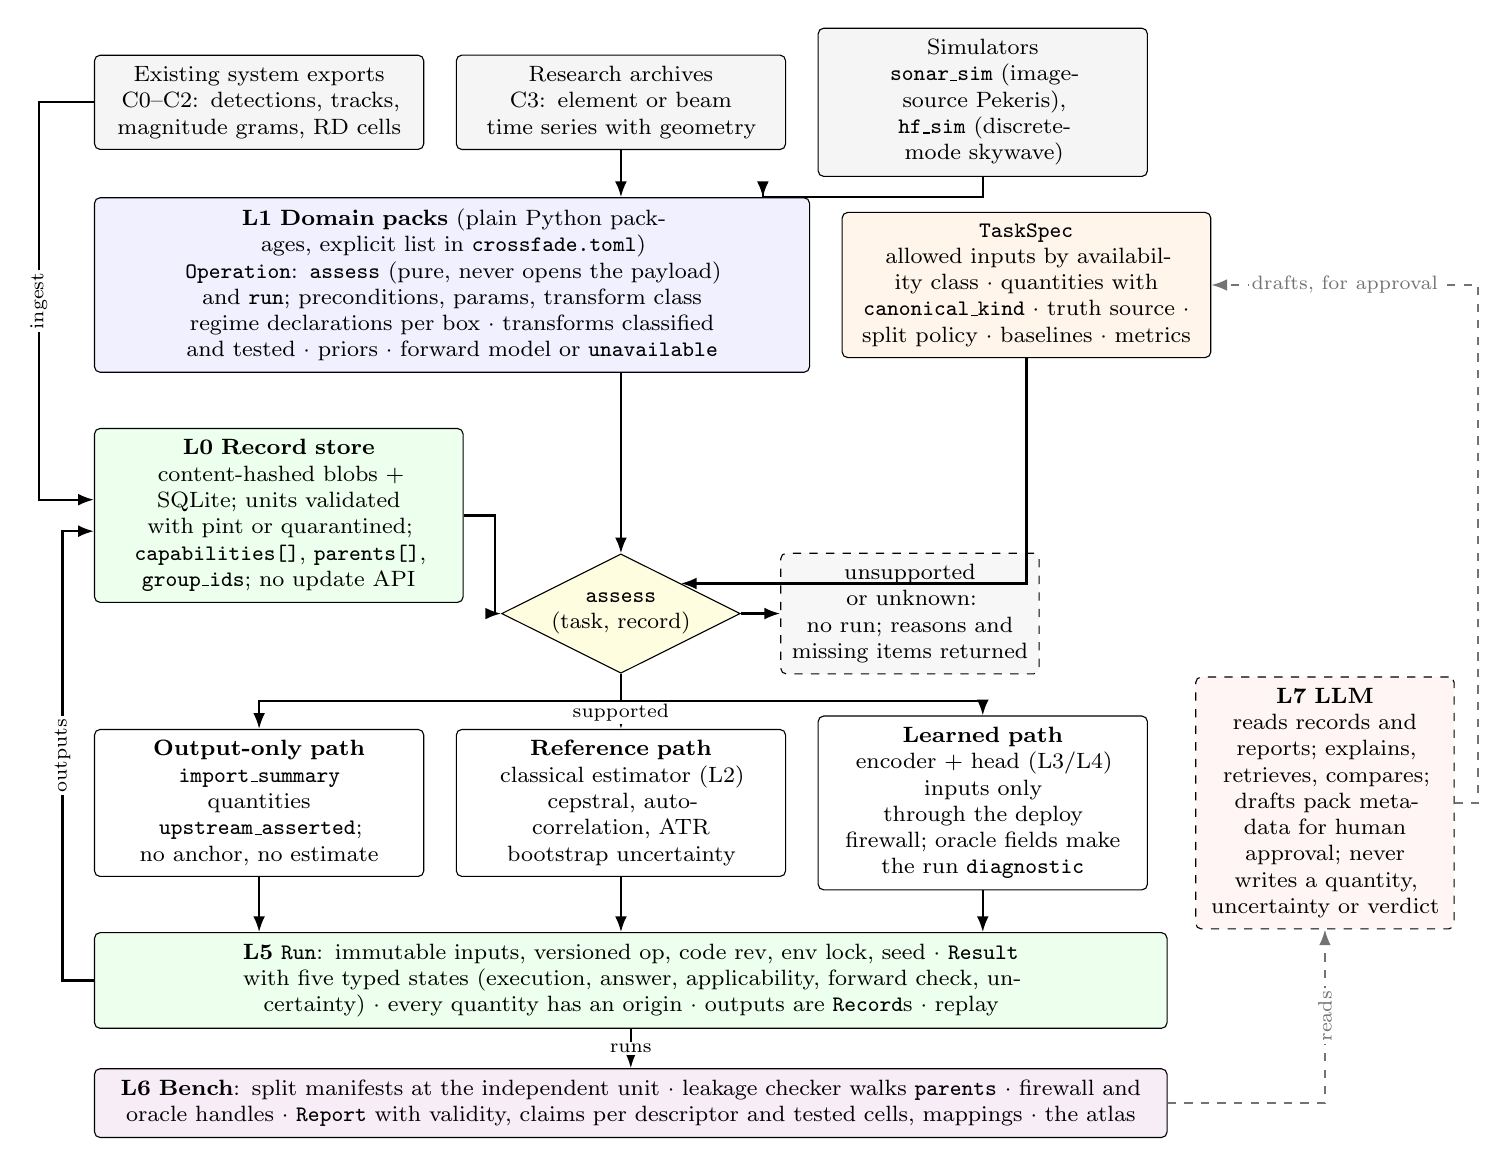
\begin{tikzpicture}[
  font=\footnotesize,
  node distance=4mm and 4mm,
  box/.style={draw, rounded corners=2pt, align=center, inner sep=4pt, minimum height=8mm, fill=white},
  src/.style={box, fill=black!4, text width=3.9cm},
  pack/.style={box, fill=blue!6, text width=8.8cm},
  task/.style={box, fill=orange!8, text width=4.4cm},
  store/.style={box, fill=green!7, text width=4.4cm},
  path/.style={box, text width=3.9cm, minimum height=13mm},
  ledger/.style={box, fill=green!7, text width=13.34cm},
  bench/.style={box, fill=violet!7, text width=13.34cm},
  llm/.style={box, dashed, fill=red!4, text width=3cm},
  dec/.style={draw, diamond, aspect=2, align=center, inner sep=1pt, fill=yellow!12},
  arr/.style={-{Latex[length=2mm]}, thick},
  darr/.style={-{Latex[length=2mm]}, thick, dashed, black!55},
  lbl/.style={font=\scriptsize, fill=white, inner sep=1pt},
  hd/.style={font=\footnotesize\bfseries},
]
% --- left column, anchored on one x ---------------------------------------
\node[store] (store) {\textbf{L0 Record store}\\content-hashed blobs + SQLite; units validated with pint or quarantined; \code{capabilities[]}, \code{parents[]}, \code{group\_ids}; no update API};
\node[pack, above=7mm of store.north west, anchor=south west] (pack) {\textbf{L1 Domain packs} (plain Python packages, explicit list in \code{crossfade.toml})\\
  \code{Operation}: \code{assess} (pure, never opens the payload) and \code{run}; preconditions, params, transform class\\
  regime declarations per box $\cdot$ transforms classified and tested $\cdot$ priors $\cdot$ forward model or \code{unavailable}};
\node[task, right=of pack] (task) {\textbf{\code{TaskSpec}}\\allowed inputs by availability class $\cdot$ quantities with \code{canonical\_kind} $\cdot$ truth source $\cdot$ split policy $\cdot$ baselines $\cdot$ metrics};

% --- sources ---------------------------------------------------------------
\node[src, above=6mm of pack.north west, anchor=south west] (s1) {Existing system exports\\C0--C2: detections, tracks,\\magnitude grams, RD cells};
\node[src, right=of s1] (s2) {Research archives\\C3: element or beam\\time series with geometry};
\node[src, right=of s2] (s3) {Simulators\\\code{sonar\_sim} (image-source Pekeris),\\\code{hf\_sim} (discrete-mode skywave)};

% --- three paths, same left edge as the store ------------------------------
\node[path, below=16mm of store.south west, anchor=north west] (p1) {\textbf{Output-only path}\\\code{import\_summary}\\quantities \code{upstream\_asserted};\\no anchor, no estimate};
\node[path, right=of p1] (p2) {\textbf{Reference path}\\classical estimator (L2)\\cepstral, autocorrelation, ATR\\bootstrap uncertainty};
\node[path, right=of p2] (p3) {\textbf{Learned path}\\encoder + head (L3/L4)\\inputs only through the deploy\\firewall; oracle fields make\\the run \code{diagnostic}};

% --- assess sits above the reference path ---------------------------------
\node[dec, above=7mm of p2.north, anchor=south] (assess) {\code{assess}\\(task, record)};
\node[box, dashed, fill=black!3, text width=3cm, right=5mm of assess] (refuse) {unsupported or unknown:\\no run; reasons and\\missing items returned};

% --- ledger, bench ---------------------------------------------------------
\node[ledger, below=7mm of p1.south west, anchor=north west] (run) {\textbf{L5 \code{Run}}: immutable inputs, versioned op, code rev, env lock, seed $\cdot$ \code{Result} with five typed states (execution, answer, applicability, forward check, uncertainty) $\cdot$ every quantity has an origin $\cdot$ outputs are \code{Record}s $\cdot$ replay};
\node[bench, below=5mm of run.south west, anchor=north west] (bench) {\textbf{L6 Bench}: split manifests at the independent unit $\cdot$ leakage checker walks \code{parents} $\cdot$ firewall and oracle handles $\cdot$ \code{Report} with validity, claims per descriptor and tested cells, mappings $\cdot$ the atlas};

% --- LLM, right of the paths row -------------------------------------------
\node[llm, right=6mm of p3] (llm) {\textbf{L7 LLM}\\reads records and reports; explains, retrieves, compares; drafts pack metadata for human approval; never writes a quantity, uncertainty or verdict};

% --- arrows ----------------------------------------------------------------
\draw[arr] (s1.west) -- ++(-7mm,0) |- node[lbl, pos=0.25, rotate=90] {ingest} ([yshift=2mm]store.west);
\draw[arr] (s2.south) -- (pack.north -| s2.south);
\draw[arr] (s3.south) -- ++(0,-2.5mm) -| ([xshift=-6mm]pack.north east);
\draw[arr] (pack.south -| assess.north) -- (assess.north);
\draw[arr] (task.south) |- (assess.north east);
\draw[arr] (store.east) -- ++(4mm,0) |- (assess.west);
\draw[arr] (assess.east) -- (refuse.west);
\draw[arr] (assess.south) -- node[lbl, pos=0.7] {supported} (p2.north);
\draw[arr] (assess.south) -- ++(0,-3.5mm) -| (p1.north);
\draw[arr] (assess.south) -- ++(0,-3.5mm) -| (p3.north);
\draw[arr] (p1.south) -- (run.north -| p1.south);
\draw[arr] (p2.south) -- (run.north -| p2.south);
\draw[arr] (p3.south) -- (run.north -| p3.south);
\draw[arr] (run.south) -- node[lbl] {runs} (bench.north);
\draw[arr] (run.west) -- ++(-4mm,0) |- node[lbl, pos=0.25, rotate=90] {outputs} ([yshift=-2mm]store.west);
\draw[darr] (bench.east) -| node[lbl, pos=0.75, rotate=90] {reads} (llm.south);
\draw[darr] (llm.east) -- ++(3mm,0) |- node[lbl, pos=0.75] {drafts, for approval} (task.east);
\end{tikzpicture}
}
\caption{The architecture. Inputs at three capability levels enter through domain packs (L1) into an immutable record store (L0). For each task, \code{assess} reads the record's declared capabilities and the task's requirements and chooses one of three paths, or refuses with reasons. All three paths write the same \code{Run} (L5) with five typed result states; the bench (L6) reads runs and writes reports and claims. The LLM (L7) reads records and reports and drafts pack metadata for human approval; it never writes a number. Physics lives entirely in the packs; the core is a ledger and a bench.}
\label{fig:architecture}
\end{figure}

\paragraph{Size budgets.} Budgets enforce the constraints. Core at end of W0: 1500 lines (review at 2500). Fixture packs: 300. \code{sonar\_sim} including the simulator: 1200. \code{hf\_sim}: 1000. \code{bench.py}: 500. W2 models: 2000. Any single function: 60. An overrun is not a failure; it is a mandatory review that asks what became a framework and whether it needed to.

\paragraph{What was rejected, and where it came from.} Regime-routed mixture-of-experts as the architecture (spec v0.1); a mandatory full-grid anchor payload from every pack (v0.1); universal PINN losses (transcript framing); the LLM inside the numerical path (transcript); thirteen record types with a \code{conditional} state (review); twelve slices with uncertainty as its own slice (review); ``no shared code'' replaced by documented independence (review; we kept both); calendar commitments removed entirely (review; we kept labelled planning estimates); xarray attributes as the unit system (v0.1); transforms as conventions (v0.1); deterministic paired views as an identifiability basis (v0.1); a \code{Mapping} written by every experiment (v0.1); H2 as a gate (v0.1); microservices, a graph database, a GNN evidence graph and a model-registry service (plan 2, v0.1).

\section{The five record types}
\label{sec:contracts}

All are Pydantic v2 models serialized to JSON. Unknown fields are rejected on load, so a contract change is a version bump, never a silent addition. Field lists are \tagP{}; the invariants in Section~\ref{sec:invariants} are \tagG{}.

\subsection{\code{Record}}
\begin{sloppypar}
Anything observed or derived: observation, representation, anchor estimate or structured summary, one type distinguished by \code{kind}. Key fields: \code{id}, \code{kind}, \code{payload\_kind} (array or structured), \code{payload\_ref}, \code{byte\_hash}, \code{manifest\_hash}, \code{source\_system}, \code{acquired\_at} (may be unknown, never inferred), \code{ingested\_at}, \code{data\_use}, \code{capability\_label} (C0--C3, a summary only), \code{capabilities[]} (explicit: \code{has\_phase}, \code{has\_array\_geometry}, \code{has\_source\_reference}, \code{has\_calibration}, \code{has\_timing}, \code{upstream\_asserted}), \code{coords}, \code{units}, \code{masks}, \code{group\_ids} (session, instrument, environment, source recording, scene; used by splits), \code{processing\_history[]} (each step with op id, version, params and transform class), \code{parents[]}, \code{produced\_by\_run}, \code{validation\_state}, \code{validation\_notes[]}, \code{regime} (per coordinate: value, units, provenance, availability, uncertainty), and \code{anchor} (required for anchor estimates: kind, descriptors each with definition and canonical kind, statistical semantics, normalization, assumptions, identifiable, ambiguous, uncertainty reference).

\end{sloppypar}
\paragraph{Identity.} \code{id} derives from the byte hash and the manifest hash together; deriving it from the manifest alone would collide for two payloads with one manifest. The manifest covers units, coordinates, masks, processing definitions and interpretation version, so identical bytes labelled seconds and milliseconds are different records. \code{produced\_by\_run} is provenance, not identity, so a replay that reproduces identical bytes and manifest reuses the record. Correcting metadata creates a successor with a parent link; the original is never edited.

\paragraph{Payloads and quarantine.} Arrays are xarray datasets with named dimensions and coordinate variables, stored as zarr. Units are validated at ingest with pint; an attribute is a label, not a check. Any unit failure, or any data variable without units, stores the record with \code{validation\_state = quarantined}; it is listable and refused by every assessment until a successor supplies what is missing.

\paragraph{Capabilities.} The C0--C3 labels remain as a summary vocabulary and never authorize anything. C0: upstream summaries (detections, tracks, scalar features; \code{upstream\_asserted}). C1: magnitude-only time--frequency views (\code{has\_timing}). C2: complex coefficients, beam-level STFT or range--Doppler cells (\code{has\_phase}, \code{has\_timing}). C3: element or beam time series with geometry. A record labelled C3 without a source reference still fails the preflight of an operation that needs one.

\paragraph{Lineage.} \code{parents[]} records derivation only, in the spirit of PROV-O without importing the ontology. Shared parents mean shared evidence and nothing more is inferred from lineage.

\subsection{\code{TaskSpec}}
\begin{sloppypar}
What a run may see and must return, loaded from YAML with the version in the filename: \code{task\_id}, \code{version}, \code{task\_kind} (transform, estimation, comparison), \code{question}, \code{allowed\_inputs[]} each with an availability class (\code{prediction\_metadata}, \code{prediction\_evidence}, \code{prediction\_estimate}, \code{training\_only}, \code{evaluation\_only}), \code{required\_capabilities}, \code{params} (each with type, units, required, \code{is\_assumption}), \code{quantities} (each with definition, units, \code{canonical\_kind} or \code{not\_channel}, \code{ambiguity\_allowed}), \code{truth\_source}, \code{normalization} (rule, reversibility, fit scope), \code{regime\_coords[]}, \code{baselines[]}, \code{metrics[]}, \code{split\_policy}, \code{uncertainty\_requirement}, \code{completion\_rule}, \code{promotion\_rule}.

\end{sloppypar}
The firewall lives here: the deploy handle returns only fields whose availability is one of the first three classes; training-only and evaluation-only fields are served through a different function, and any run that receives them is tagged \code{diagnostic}. Assumptions are parameters: a physical assumption an operation needs is a parameter with \code{is\_assumption = true}; if absent, \code{assess} returns \code{unsupported} naming it. Nothing is ever assumed on the caller's behalf.

\subsection{\code{Operation}}
\begin{sloppypar}
A pack's executable unit, a protocol: \code{op\_id}, \code{version}, \code{preconditions[]} (capabilities the record must carry), \code{params\_model} (unknown params refused), \code{transform\_class} (exact, coordinate, lossy, physical, none), \code{determinism} (exact or tolerance), \code{is\_model}, and two methods. \code{assess(task, record, params)} is pure and fast: it reads capabilities, validation state, units, coordinates, processing history and params, never the payload, and returns \code{supported}, \code{unsupported} or \code{unknown} with named reasons and missing items. Value-level checks (a nonfinite unmasked sample, zero total weight) therefore happen in \code{run} and produce \code{answer = unsupported} with reasons in diagnostics while the run itself succeeds. The registry reads the explicit pack list, imports each module, checks \code{CORE\_API\_VERSION == 1}, and fails whole on any error; there is no partial registry.

\end{sloppypar}
\subsection{\code{Run}}
\begin{sloppypar}
One execution attempt: \code{run\_id}, task and op with versions, \code{inputs[]}, \code{params}, \code{assumptions\_used}, \code{code\_rev}, \code{env\_lock\_hash}, \code{seed}, \code{path} (reference, learned, output\_only, diagnostic), timestamps, \code{status} (succeeded, failed, cancelled), \code{attempt\_of}, \code{error}, and a \code{result} holding \code{quantities} (each with value, units and origin: \code{upstream\_asserted}, \code{computed}, \code{inferred}), \code{outputs[]}, and the typed states of Section~\ref{sec:states}. Publication order: output records first, then the run JSON, then the SQLite row, each via temp file and atomic rename; a crash between steps leaves orphan outputs that \code{verify} reports, never a run referencing missing outputs. \code{replay} re-resolves the op by id and version, re-executes with the same inputs, params and seed, compares by the determinism contract, and records a new run with \code{attempt\_of} set.

\end{sloppypar}
\subsection{\code{Report}}
One declared comparison: an \code{ExperimentSpec} (task, data manifests with roles, arms with exposure, primary metric, effect rule with a frozen timestamp, seeds, tuning policy, budgets, \code{exploratory} flag), a \code{SplitManifest} (unit, partitions, frozen timestamp, hash), \code{runs[]}, per-arm metrics with intervals and denominators, observed budgets, \code{validity} (valid, invalid, incomplete), deviations, \code{claims[]} and \code{mappings[]}. A \code{Claim} names direction, descriptor, the regime cells actually tested, arm and baseline arm, outcome (supported, evidence\_against, inconclusive), effect with interval, and limitations. A \code{Mapping} is recorded only for an implemented correspondence. Claims are written only from valid reports; a failed arm is a failed run and never evidence against anything.

\section{Invariants}
\label{sec:invariants}

Each has a test; the slice column names where it is first enforced. All \tagG{}.

{\small
\begin{longtable}{@{}lp{11.5cm}l@{}}
\toprule
Id & Invariant & Slice \\
\midrule
\endhead
CF-01 & Payload blobs are written once and never modified; there is no update path & W0 \\
CF-02 & Record identity covers payload bytes and semantic manifest; same bytes with different units are different records & W0 \\
CF-03 & Every array record has validated units on every data variable and coordinate, or is quarantined & W0 \\
CF-04 & A capability label never authorizes an operation; \code{assess} checks explicit capabilities and params & W0 \\
CF-05 & \code{assess} returns \code{unknown} when prerequisites cannot be established; \code{unknown} is never coerced to \code{supported} & W0 \\
CF-06 & A task fixes allowed inputs by availability class; the deploy handle cannot return training-only or evaluation-only fields & W0 \\
CF-07 & An anchor estimate may omit its payload; no field is fabricated to satisfy a shape & W0 \\
CF-08 & A deterministic transform reports uncertainty \code{not\_applicable}; a learned estimate without validated uncertainty reports \code{unavailable}; neither is ever a number & W0 \\
CF-09 & A forward check with no forward model is \code{unavailable}, never \code{passed} & W0 \\
CF-10 & Every run resolves to immutable inputs, a versioned op, a code revision and an environment lock & W0 \\
CF-11 & Failed and cancelled runs are persisted and linked; a retry is a new run with \code{attempt\_of} & W0 \\
CF-12 & Outputs are published before the run that references them & W0 \\
CF-13 & Every quantity carries an origin: \code{upstream\_asserted}, \code{computed} or \code{inferred} & W0 \\
CF-14 & Splits are at the declared independent unit; every derived record inherits its root's group ids; the checker refuses a partition crossing & W1 \\
CF-15 & Oracle-provenance regime coordinates and evaluation-only fields never reach a run on the learned or reference path; a run that uses them is diagnostic & W1 \\
CF-16 & Test membership is frozen before any pretraining; unlabeled test exposure is recorded as exposure & W2 \\
CF-17 & A valid negative or inconclusive report completes an experiment; an invalid or incomplete report produces no claim & W1 \\
CF-18 & Every claim names its arm, baseline arm, direction, descriptor, regime cells tested, effect and budgets & W1 \\
CF-19 & Tested support is the list of evaluated cells; the atlas never marks an untested interior cell validated & W1 \\
CF-20 & Shared-parent results are one piece of evidence; unknown model dependence withholds numerical fusion & W3 \\
CF-21 & No pack operation writes to an upstream system & W3 \\
CF-22 & Anchor-estimate uncertainty is propagated or the result is tagged \code{conditional\_on\_plugin} naming the estimate & W1 \\
CF-23 & Every quantity in a task names a \code{canonical\_kind} or is tagged \code{not\_channel} & W0 \\
CF-24 & Every transform in a pack has a class and an equivalence test & W1 \\
CF-25 & Unknown fields on any record type are rejected on load & W0 \\
\bottomrule
\end{longtable}}

\section{Domain packs}

A domain pack is a plain Python package exposing a manifest and operations. The core registers packs from an explicit list; the platform owns execution, records and evaluation; the pack owns domain meaning. \tagG{} for the boundary; \tagP{} for the element list: \code{manifest} (name, version, core API version, operation ids, fixtures), \code{operations[]} (at least one), \code{regime} (declared ranges per group, placeholder or measured; canonical anchor kind per box), \code{transforms} (every transformation applied or admitted, classified and tested), \code{tests} (golden fixtures, known failure cases, regime boundaries where a method stops working), and optionally \code{priors}, \code{forward\_model} (declared \code{unavailable} when absent), \code{anchor\_estimators} and \code{vocabulary}.

\paragraph{Transform classification.} Under the generative model~\eqref{eq:generative}:
\begin{center}\small
\begin{tabular}{@{}p{2.6cm}p{4.2cm}p{3.6cm}p{4cm}@{}}
\toprule
Class & Examples & Expected behaviour & Test \\
\midrule
Exact convention & Unit relabel, sample-index origin, complex sign convention & Invariant & Output identical after inverse conversion \\
Coordinate transform & Array rotation, beam steering, reference-frame change & Equivariant & Output transforms by the declared rule \\
Lossy processing & Resampling, window length and overlap, magnitude-only, decimation, CFAR thresholding & Declared information loss; applicability may change & Retained-information contract stated and checked on fixtures \\
Physical intervention & Carrier retune, sound-speed change, ionospheric state change, source motion & Answer may change & Not an invariance; recorded as a context change \\
\bottomrule
\end{tabular}
\end{center}

\paragraph{Passive sonar pack, sketch.} Operations: beamform-and-STFT (lossy, parameters recorded), cepstral arrival estimation, ray-based blind deconvolution, striation-slope estimation, later a learned descriptor estimator, each declaring preconditions (array geometry, sound speed at the array, band). Regime: $M$ up to $10^{-2}$, $\betaB$ up to $1$, $\Pif$ 1 to 50, placeholders. Canonical kind: \code{delay\_scale} when $\Pis$ exceeds the declared threshold, else \code{delay\_doppler}. Priors: sparse ray arrivals with surface and bottom images; approximately linear modal phase in frequency for low-order modes; waveguide-invariant striation slope. Forward model: the image-source generator of Section~\ref{sec:pekeris}; a normal-mode or ray model later; a neural-operator surrogate of a parabolic-equation solver is a later option \citep{kovachki2023}.

\paragraph{HF skywave pack, sketch.} Operations: matched filter and Doppler processing (lossy), multimode delay--Doppler estimation from range--Doppler cells, sparse CIR reconstruction under interference. Regime: $M$ around $10^{-6}$, $\betaB$ around $10^{-2}$, $\Pin$ set by ionospheric coherence time. Canonical kind: \code{delay\_doppler}. Priors: few discrete modes with ordinary and extraordinary splitting; slow multiplicative fading; mode delay ordering. Forward model: the discrete-mode generator of Section~\ref{sec:hf}; a published ray tracer once its license and callable form are verified.

\paragraph{Output-only pack.} A legacy system connects with one operation, \code{import\_summary}, no forward model and no anchor estimator. It participates in comparison and lineage warnings, and every request for reconstruction returns \code{unsupported} with the missing capabilities named. This is how existing programmes join without touching their processing chains, and it ships independently of any transfer result.

% =====================================================================
\part{Estimators, models and the training objective}

\section{Anchor estimators}

Every anchor estimator states what it can and cannot recover from its inputs (Section~\ref{sec:ident}). A capability label never authorizes an estimator; its own \code{assess} checks its preconditions and refuses with the missing items named.

\begin{center}\small
\begin{tabular}{@{}p{3.4cm}lp{3.4cm}p{3.6cm}p{2.6cm}@{}}
\toprule
Estimator & Level & Recovers & Assumes & Ambiguous \\
\midrule
Striation slope, waveguide invariant $\beta$ & C1 & Range-rate to range ratio, mode interference structure & Few-mode waveguide, broadband source & Absolute range without a frequency anchor \\
Cepstral multipath & C1/C2 & Relative arrival delays, boundary reflection structure & Dominant first arrival, arrivals separable in quefrency & Arrival ordering; delays within one cell \\
Artificial or synthetic time reversal & C3 & Source waveform and source-to-array impulse response & Linear modal phase, known geometry and local sound speed & Overall delay and scale \\
Ray-based blind deconvolution & C3 & Impulse response and source waveform, broadband & Resolvable ray arrivals, known geometry & Source spectrum absolute level \\
Bilinear models for sources of opportunity & C3 & Channel from unknown but structured sources & Source in a known low-dimensional subspace & Source--channel split within the subspace \\
Wideband ambiguity, Mellin-domain scale & C2/C3 & Scale $\alpha$ and delay $\tau$ jointly & Known or estimated source, wideband regime & Sign of scale for symmetric spectra \\
Delay--Doppler multimode & C2 & Mode delays and Dopplers & Narrowband regime, few discrete modes & Ordinary--extraordinary assignment \\
Sparse CIR reconstruction under interference & C2 & Full-band CIR from partial spectrum & Sparse arrivals, temporal smoothness & Arrivals within one resolution cell \\
\bottomrule
\end{tabular}
\end{center}

\paragraph{Learned estimators.} Trained on the pack's forward model with the same structural priors as losses (sparsity in delay, smoothness in time, forward consistency through $\mathcal M_d$), following the physics-informed transformer precedent that reached power-delay-profile similarity $0.82$ against $0.62$ for the best baseline at fifty percent spectrum occupancy \citep{zubow2026}. A learned estimator inherits the classical estimator's assumption list and declares its training regime box. An estimated anchor used as a training target is a \code{pseudo\_label} and the record says so.

\paragraph{Estimator output.} An anchor record: a kind, an optional payload, named descriptors as functionals of the canonical kind, statistical semantics, and the three lists \code{assumptions}, \code{identifiable}, \code{ambiguous}. A downstream head that needs an ambiguous quantity returns a distribution over the alternatives or abstains.

\paragraph{Out of scope here.} Detection, classification and tracking heads sit on top of results and are owned by each programme's existing systems or by later task-specific work.

\section{Models}

The first learned candidate is a dense shared/private encoder with domain adapters \citep{bousmalis2016}, trained only after the baseline ladder of Section~\ref{sec:transfer} has been run. Regime-routed mixture of experts is an ablation arm, not the architecture. \tagP{} for the candidate; \tagH{} for every claim that one arm beats another.

\paragraph{Why routing is demoted.} The 2026 result that motivated it covers two fluid regimes and reports domain-separated routing with low validation error \citep{sharma2026}. That is evidence routing can avoid gradient conflict between incompatible regimes; it is not evidence that routing is best for inverse channel tasks, and a router fed regime coordinates that trivially predict the target is not discovering physics. The 2026 benchmark showing physics foundation models to be conditional generalists with negative transfer in a substantial fraction of cases \citep{chu2026} is why the from-scratch arm is mandatory.

\paragraph{Losses.} Each is individually validated in the literature; their composition is the hypothesis.
\begin{center}\small
\begin{tabular}{@{}p{2.8cm}p{3.4cm}p{3.8cm}p{4.2cm}@{}}
\toprule
Loss & Form & Views or inputs & Claim it supports \\
\midrule
L1 Masked modelling & Reconstruct masked patches of the native view & Unlabeled archives per domain & Label-free pretraining, as in masked spectrogram modelling for radio and the RF foundation models \\
L2a Representation consistency & Contrastive between deterministic re-representations of one recording & Same recording, deterministic transforms & Encoder consistency across representations \citep{jiang2026}; not identifiability \\
L2b Content isolation & Contrastive between views with independent nuisance variation & Sub-arrays of one event; time windows of a stationary source; different upstream chains; controlled simulation pairs & Isolation of shared physical content up to an invertible map \citep{vonkugelgen2021,gresele2020}; the alignment basis \\
L3 Cross-domain anchor alignment & Contrastive between shared latents of records from different domains whose canonical-kind descriptors match, restricted to the descriptor's overlapping regime box & Descriptor-matched pseudo-pairs, tagged as such & Sharing where physics says it may exist; never whole-domain alignment \citep{zhao2019} \\
L4 Structural physics & Arrival sparsity in $\tau$, temporal smoothness of $h$, forward consistency where $\mathcal F_d$ exists & Anchor estimates & The physics-informed part that applies to channels \citep{zubow2026,sabra2004} \\
L5 Transform consistency & Invariance under exact conventions only; equivariance under coordinate transforms; tested behaviour under lossy processing & Pack transform declarations & The transform classification \\
L6 Private preservation & Reconstruct native view from shared and private latents; orthogonality penalty & All & Domain detail retained \citep{bousmalis2016} \\
\bottomrule
\end{tabular}
\end{center}

\paragraph{Pretraining plan.} L1 begins once the split policy and transform contracts are frozen and test membership is fixed; ``unlabeled'' does not exempt data from exposure rules. L2a and L4 follow once anchor estimates exist. L2b requires paired views from the pairing protocol. L3 runs only at declared regime overlap per descriptor. L5 and L6 throughout. Task heads last.

\paragraph{Budgets.} Adaptation efficiency (target labels, target unlabeled exposure, adaptation compute) and total cost (simulation, pretraining, tuning, inference) are two separate views, always both. For any sparse arm, active and total parameters are both reported.

\paragraph{Not the objective.} Latent overlap, embedding visualizations, and domain indistinguishability under a discriminator are not success criteria.

\paragraph{What transfers today, in these domains.} ImageNet-pretrained vision models slightly beat audio-pretrained networks on passive sonar target recognition: what transferred was spectrogram texture, not acoustics \citep{mohammadi2024}. Masked-autoencoder pretraining on communications I/Q transferred to radar signal recognition with a one-shot gain close to in-domain pretraining \citep{huang2025}. CSI-CLIP++ transferred an RF channel encoder across three tasks and across simulators under ideal ray-traced CSI \citep{jiang2026}. The pattern: shallow transfer from generic image pretraining is easy and weak; deeper transfer appears when the objective is built on paired physical views of the channel. The domain-expert tier is being built by others (RF foundation models; an underwater acoustic foundation model under contract). The differentiated contribution is the anchor, the regime atlas and the evidence layer.

% =====================================================================
\part{Inference, uncertainty and typed states}

\section{Typed result states}
\label{sec:states}

Every result carries five independent state fields. No single Boolean stands in for them, and no state is ever filled by default with a passing value. \tagG{}

\begin{center}\small
\begin{tabular}{@{}p{2.2cm}p{5.6cm}p{6.2cm}@{}}
\toprule
Dimension & States & Rule \\
\midrule
Execution & succeeded, failed, cancelled & A failed run publishes no quantities \\
Answer & complete, partial, abstained, unsupported & partial names what is missing \\
Applicability & in\_scope, out\_of\_scope, unknown & unknown is the default, never in\_scope \\
Forward check & passed, failed, unavailable, not\_applicable & Absent forward model means unavailable, never passed \\
Uncertainty & posterior, confidence\_interval, predictive\_interval, ensemble\_summary, unavailable, not\_applicable & A deterministic transform is not\_applicable; a learned estimate without validated uncertainty is unavailable \\
\bottomrule
\end{tabular}
\end{center}
Each quantity is tagged \code{upstream\_asserted}, \code{computed} or \code{inferred}, so a consumer can tell a legacy system's own confidence from a Crossfade estimate.

\section{Inference methods}

Not one algorithm. A deterministic transform returns a value. A classical estimator returns a value and whatever error characterization its literature supports; in W1, a block bootstrap over time segments. Where a pack has a forward model and a prior, simulation-based inference is the preferred route to a posterior: train a neural posterior estimator on $(\theta,\ \mathcal M_d[\mathcal F_d(\theta)]+\varepsilon)$ pairs and amortize on real observations, using the \code{sbi} library before anything custom, with the diagnostics the guides prescribe \citep{deistler2025,dax2026}. SBI is a method a pack may use, not a return type the platform demands.

\paragraph{Forward validation.} Where $\mathcal F_d$ and $\mathcal M_d$ exist, the engine predicts what the pack would observe under the inferred explanation and compares at the observation level actually available. A check on data that trained the estimator is labelled in-sample. Agreement is necessary and not sufficient; when the posterior is multimodal or an ambiguous quantity is involved, \code{alternatives[]} is populated.

\paragraph{Uncertainty record.} Beyond its kind, an uncertainty carries the estimand, the conditioning information, the method and version, and the population and regime box on which it was validated. A result that plugs in a point anchor estimate says \code{conditional\_on\_plugin} and names the estimate; otherwise the anchor's own uncertainty is propagated. Post-hoc calibration degrades under shift \citep{ovadia2019} and conformal guarantees hold under exchangeability or specific departures, so applicability is reported alongside every uncertainty and \code{unknown} is a legitimate value.

\paragraph{Abstention.} A head may abstain when applicability is out of scope or unknown, or when a forward check fails a declared threshold. Abstentions are runs with \code{answer = abstained}, so the abstention rate is a metric with a denominator.

\paragraph{Fusion.} The two rules of Section~\ref{sec:transfer} and nothing more until a use case exists.

% =====================================================================
\part{Evaluation protocol}

\section{Three levels of demonstration}

\begin{center}\small
\begin{tabular}{@{}lp{6.6cm}p{4.4cm}@{}}
\toprule
Level & Shows & Does not show \\
\midrule
E0 Contract fixture & T0 computes a known property of a supplied profile; storage, units, capability handling, replay work & Anything about channels or transfer \\
E1 Within-domain estimation & A declared descriptor is estimated from permitted observations and compared to independent truth with its own error model; classical and from-scratch baselines characterized & Transfer \\
E2 Cross-domain transfer & Only the declared transfer intervention changes; target utility measured under held-out conditions; shared-simulator smoke tests, independent-domain evidence and measured-data validation reported separately & Universal generalization \\
\bottomrule
\end{tabular}
\end{center}
An E0 result is never promoted to E1 or E2 by relabelling data.

\section{Preregistration, firewall, splits, pairing}

\paragraph{Preregistration.} An experiment is confirmatory only if every field is filled: task version, data manifests, roles, arms with exposure, primary metric, effect rule with a frozen timestamp, seeds, tuning policy, budgets, independent unit, expected failure modes, exclusions. A spec missing any of these may run as exploratory and produces no claim. No universal percentage threshold is invented; baseline variability is estimated on development data, the meaningful effect is agreed, and the rule is frozen before the locked test is viewed.

\paragraph{Feature and truth firewall.} Every input field has one availability class. The deploy handle serves only prediction-time fields. Oracle fields are served by a separate function and any run that calls it is diagnostic and cannot satisfy the promotion gate. Anchor estimates used for pairing are pseudo-labels carrying estimator version, lineage and uncertainty. Test reference answers never choose routing, positive pairs or normalizers on the deploy path. In simulation this is the main leakage risk: a coordinate computed from the simulator's true delay spread, feeding a model whose target is delay spread, is the answer in disguise.

\paragraph{Splits and exposure.} At the task's independent unit: session, environment, instrument, scene or source recording. Every derived record inherits its root's group ids; the checker walks parents to the root and refuses a partition crossing. Test membership is frozen and hashed before any pretraining. Target-domain unlabeled exposure is recorded per arm. Normalization, regime selection, pairing thresholds and calibration are fit on training or training-plus-development partitions only.

\paragraph{Pairing.} Each pair record declares one basis: \code{same\_event} (two instruments observed one physical event), \code{controlled\_mechanism} (two independent simulators rendered a deliberately corresponding mechanism), \code{descriptor\_matched} (pseudo-pair by matching estimated descriptors; weakest), or \code{negative}. They are never pooled. Shuffled-pair and nuisance-matched controls run where the task's shortcut risks call for them.

\paragraph{Simulator independence.} A cross-domain claim from simulation requires both no shared forward-physics kernel and a written independence statement covering scene distribution, approximation family and truth construction. Code independence is the cheap auditable proxy; assumption independence is the target; neither substitutes for the other or for measured-data validation.

\section{Gates}

\begin{center}\small
\begin{tabular}{@{}lp{4cm}p{5.2cm}p{3cm}@{}}
\toprule
Gate & Question & Passes when & Does not imply \\
\midrule
Delivery & Did the declared arms run validly and reproducibly? & Required arms present; leakage checks pass; report rebuilds from persisted runs & Any scientific result \\
Scientific & What does the result support? & A scoped claim with effect, interval, budgets and limitations, in any direction & Deployment fitness \\
Promotion & Is the model useful for its declared inputs? & Preregistered utility and uncertainty criteria met at the independent unit on relevant data & Anything beyond tested cells \\
\bottomrule
\end{tabular}
\end{center}
An experiment is complete when a preregistered comparison ran validly and produced a report. A model is promoted when the report supports its declared utility. A hypothesis is supported, contradicted, or inconclusive. None of the three implies another.

% =====================================================================
\part{Build plan}

\section{Slices}

Four slices ship now and three wait for a reason to exist. Each is a complete user-visible operation with a demo and a test suite. Estimates are planning numbers for the funding conversation, labelled as such, and assume the sonar lead's W1 input arrives in the first two weeks. \tagP{}

\begin{center}\small
\begin{tabular}{@{}p{2.2cm}p{5cm}p{2.6cm}p{2.2cm}p{2.4cm}@{}}
\toprule
Slice & Deliverable & Gate & Estimate & Blocked by \\
\midrule
W0 Workbench & Ingest a supplied profile; compute T0; preserve units and lineage; replay; refuse reconstruction on a summary record & Delivery & 2--3 weeks, one engineer & Nothing \\
W1 First task & Simulated beam time series from the image-source waveguide; RMS delay spread and arrival count via cepstral and autocorrelation estimators; bootstrap uncertainty; bench with grouped splits and leakage checks; a report characterizing the classical estimators & Delivery and scientific & 4--6 weeks, two people & Sonar lead confirms the quantity and the simulator \\
W2 Transfer charter & HF pack with an independent multimode simulator; SSL arm; dense shared/private arm; one preregistered transfer trial per descriptor with typed uncertainty & Scientific, any direction & 8--12 weeks, two to three people & W1 split policy frozen; pairing basis; independence statement \\
W3 Output-only adapter & Read-only import of one existing system's summary export; comparison; duplicate-evidence warnings; no upstream write & Delivery & 2--3 weeks, parallel to W1 & Which system and export format \\
Later: routing & Dense versus routed ablation & After W2 shows a dense arm worth beating & Deferred & W2 result \\
Later: explanations & LLM over records; pack-metadata drafts for approval & After W1 records are stable & Deferred & Stable Run and Report \\
Later: fusion & Numerical combination under a declared dependence model & After a use case exists & Deferred & A use case \\
\bottomrule
\end{tabular}
\end{center}

\paragraph{Dependencies.} W0 and W3 share \code{Record} and \code{Run} and nothing else. W1 shapes the contracts alongside W0 and starts the day its quantity is confirmed. W2 depends on W1's split policy for its pretraining start and on W1's estimators for its baselines.

\paragraph{What each gate refuses.} W0: any anonymous tensor; any record without explicit capabilities; any fabricated default for a missing unit, reference scale or convention; any assessment that coerces unknown to supported. W1: any learned-arm result without ladder arms 1 and 2; any random-window split; any oracle coordinate on the reference or learned path; any estimator without a typed uncertainty or an explicit unavailable. W2: any gain measured on one simulator relabelled; any missing independence statement; any pretraining before test membership is frozen; any calibration claim validated only on the training cells; any claim from an invalid or incomplete report. W3: any write to upstream processing; any duplicate evidence counted twice; any upstream confidence relabelled as a Crossfade estimate.

\paragraph{Team.} One person on packs and estimators (the sonar lead's domain), one on the core and bench, and from W2 one on models.

\section{W0: the workbench, as built}

Implemented test-first on branch \code{w0-workbench}: five core modules (\code{records}, \code{tasks}, \code{packs}, \code{runs}, \code{db}) plus the CLI, two fixture packs, two task specifications, the golden fixture, and 39 tests mapped one-to-one to the PRD's acceptance tests; ruff clean; core at 804 lines against a 1500-line budget. Three details settled during implementation are reflected in the contracts: value-level checks live in \code{run}, not \code{assess}; \code{Record.id} derives from both hashes; \code{produced\_by\_run} and \code{validation\_notes} were added. The worker runs in-process; subprocess isolation with a resource limit is the next increment and changes no contract. The branch is not merged pending the sonar lead's review of the architecture.

\section{W1: the first real task}

\paragraph{Task specifications.} \code{pdp.rms\_delay\_spread} and \code{pdp.arrival\_count}, both estimation tasks. Allowed inputs: beam time series (prediction evidence); sampling rate, band, array geometry, local sound speed (prediction metadata); the arrival list (evaluation only); simulator parameters (training only). Required capabilities: \code{has\_timing}, \code{has\_phase}. Parameters: window length (lossy, recorded), cepstral lifter, \code{assume\_point\_source} (an assumption). Quantities: RMS delay spread in seconds and arrival count, both with canonical kind \code{power\_statistic}, the count with ambiguity allowed. Truth: exact functionals of the arrival list. Regime coordinates: $\Pit$ (inference, estimated; and oracle for diagnostics), $\Pif$ (inference, from band and depth if supplied), $\mathrm{SNR}_{\mathrm{cell}}$ (estimated). Split policy: unit is the scene; held-out groups are scene and environment. Uncertainty: ensemble summary or predictive interval, never unavailable.

\paragraph{Regime grid.} Water depth $\{50,100,200\}$~m; range $\{1,3,10\}$~km; bottom $\{$sand, silt, rock$\}$ as sound speed and density pairs; centre frequency $\{200,500,1000\}$~Hz with fractional bandwidth $\{0.3,0.6\}$; SNR per cell $\{-10,0,10\}$~dB: 486 cells, three scenes per cell with different source and receiver depths. Cells are the atlas's tested support.

\paragraph{Operations.} \code{beamform\_stft} (lossy; declares the window length and ships a test that delay spread from two window lengths agrees within a declared tolerance on the golden scene); \code{autocorr\_pdp} (anchor kind \code{power\_statistic}, PDP on a delay grid plus the two descriptors; block bootstrap); \code{cepstral\_pdp} (kind \code{descriptors\_only}; block bootstrap); \code{direct\_from\_truth} (diagnostic path). Each estimator lists \code{identifiable = [rms\_delay\_spread]} and \code{ambiguous = [arrival\_count within one cell]}.

\paragraph{Experiment W1-E1.} Arms: the two estimators and the diagnostic sanity arm. Primary metric: absolute error in RMS delay spread in resolution cells, per scene. Secondary: arrival-count error under the stated merging rule; bootstrap coverage at the nominal level; abstention rate below a declared SNR floor. Effect rule: characterization, not superiority; per-cell error and coverage tables. Seeds: five. Claims: one per estimator per descriptor, supported if coverage is within tolerance across tested cells, else evidence against with the failing cells listed. These are claims about the estimator's error model, not about transfer. Definition of done: ten acceptance tests green, a report in the store, and a one-page summary for the sonar lead of which cells each estimator is trustworthy in.

\section{W2: the transfer charter}

\paragraph{Software.} \code{packs/hf\_sim} with the discrete-mode simulator, an \code{import\_rangedoppler} lossy transform, a \code{multimode\_dd} estimator producing a \code{delay\_doppler} anchor with the two descriptors, and a bootstrap uncertainty; an independence statement stored as a record; model operations in each pack for ladder arms 2 to 6, all reading inputs through the deploy firewall; pairing records with a declared basis (primary \code{controlled\_mechanism}: for each cell in the overlap the two simulators render scenes whose PDP descriptors are deliberately matched; secondary \code{descriptor\_matched}, never pooled); the regime coverage report produced before any transfer run.

\paragraph{Arms and budgets.}
\begin{center}\small
\begin{tabular}{@{}p{5cm}lp{3.2cm}ll@{}}
\toprule
Arm & Ladder & Pretrained from & Target labels & Target unlabeled \\
\midrule
A1 classical & 1 & none & 0 & 0 \\
A2 features + head & 2 & none & $N$ & 0 \\
A3 scratch & 3 & none & $N$ & 0 \\
A4 target SSL & 4 & target unlabeled & $N$ & all train \\
A5 pooled & 5 & both, labeled & $N$ & all train, both \\
A6 dense shared/private, source-pretrained & 6 & source SSL then source labeled & $N$ & source all; target 0 \\
A6$'$ dense shared/private, source + target SSL & 6 & source and target SSL & $N$ & all train, both \\
\bottomrule
\end{tabular}
\end{center}
Learning curve $N\in\{8,32,128,512\}$ target scenes. Controlled: target labels, adaptation compute, tuning budget. Reported: upstream pretraining compute, total parameters. Seeds: five. Independent unit: scene, held out by scene and environment.

\paragraph{Effect rule, to be frozen before the locked test.} Primary metric as in W1. Effect $\delta(N)=L_{\mathrm{A3}}(N)-L_{\mathrm{A6}}(N)$. Meaningful $\delta_{\min}$: the smallest delta exceeding two seed standard deviations of A3 on the development set at $N=32$, frozen and timestamped before the test partition is read. Decision as in Section~\ref{sec:transfer}.

\paragraph{Shortcut controls.} Shuffled-pair control (A6 with pairing bases permuted; a gain surviving this is not transfer); nuisance-matched control (target scenes matched on SNR and bandwidth only); oracle-regime diagnostic (A6 given oracle $\Pit$; diagnostic path; cannot promote). The predicted negative control is a Doppler-spread descriptor added to both packs if time allows.

\paragraph{Open inputs that block the scientific gate, not the software.} Pairing-basis approval (sonar lead); HF simulator simplification acceptance (an HF-familiar reviewer); whether the W1 error model is tight enough in the overlap cells to serve as pseudo-label truth for A6$'$ (numerical reviewer); a named measured dataset for the reality check (sonar lead).

\section{W3: the output-only adapter}

One pack with two operations: \code{import\_summary} parses an existing system's export into summary records with origin \code{upstream\_asserted}, the system's confidence kept in diagnostics and never under uncertainty, and group ids from whatever session or file identifiers the export carries; \code{compare\_summaries} aligns two summary records on time and declared keys, lists agreements and disagreements, and warns when both resolve to the same parents. Non-goals: any estimate, any anchor, any learned op, any numerical fusion, any write to the upstream system, any live connection. A static check confirms no file writes outside the store. Blocked only by which system and which export format (ADR-25).

\section{Data and simulators}

Nothing is invented as available. The two in-house generators are specified in Sections~\ref{sec:pekeris} and~\ref{sec:hf}. Public candidates for the reality gate, each with what must be verified before use: SWellEx-96 (current hosting and terms; which arrays and events are public; source-track resolution); SBCEX17 ship-noise recordings (whether the recordings or only derived products are public); DeepMIMO (simulated, so it serves the independent-generator check, not the reality gate); a measured indoor or vehicular time-varying CIR dataset with enough sessions for grouped splits (to be identified). Programme data enters only at W3 through the output-only adapter unless C3 archives are already cleared for research use; every record carries the owner's \code{data\_use} label; nothing assumes a new collection campaign. Every dataset is described by a manifest record (source, license or clearance, capabilities, group-id scheme, truth kind and error model, regime coverage as a list of cells, known gaps) before any run consumes it, and the bench produces from the manifests the per-descriptor regime coverage and intersection before any transfer hypothesis runs.

\section{Decision register}

{\small
\begin{longtable}{@{}lp{7.4cm}lp{2.6cm}p{2cm}@{}}
\toprule
Id & Decision and choice & Tag & Status & Blocks \\
\midrule
\endhead
ADR-01 & Product unit: capability-aware task execution with an auditable ledger; transfer is a measured extension & P & Adopted & -- \\
ADR-02 & Five record types & P & Adopted & -- \\
ADR-03 & Anchor as a typed family with optional payload; descriptors as functionals of a canonical kind; canonical kind per regime box & P & Adopted & -- \\
ADR-04 & Three execution paths chosen by assess; no planner, no DAG engine & P & Adopted & -- \\
ADR-05 & Explicit capabilities plus per-op preconditions; C0--C3 as labels only & G & Adopted & -- \\
ADR-06 & Assumptions are parameters; no conditional state & G & Adopted & -- \\
ADR-07 & Content-hashed files plus SQLite; zarr for arrays; JSON for structured & P & Adopted & -- \\
ADR-08 & pint validation at ingest; quarantine on failure & G & Adopted & -- \\
ADR-09 & Explicit pack list; one core API version integer & G & Adopted & -- \\
ADR-10 & First scientific task: RMS delay spread and arrival count from beam time series, simulated, C3 & P & Proposed, awaiting sonar lead & W1 \\
ADR-11 & W1 simulator: in-house image-source Pekeris waveguide; refraction-capable code as second generator later & P & Proposed, awaiting sonar lead & W1 \\
ADR-12 & Truth exact from the arrival list in W1; estimated anchors are pseudo-labels everywhere & G & Adopted & -- \\
ADR-13 & Regime coordinates task-scoped, provenance-bearing, nullable, with availability; per-descriptor matching & G / H & Adopted & -- \\
ADR-14 & First learned arm: dense shared/private with adapters after ladder arms 1--5; routing optional & P & Adopted & W2 \\
ADR-15 & SSL starts when W1's split policy is frozen and test membership hashed & G & Adopted & W2 \\
ADR-16 & Typed uncertainty kinds; block bootstrap for classical estimators in W1 & G / P & Adopted & -- \\
ADR-17 & Forward checks only where a pack declares a forward model & G & Adopted & -- \\
ADR-18 & Report holds claims; Mapping only for implemented correspondences; tested cells listed & G & Adopted & -- \\
ADR-19 & Simulator independence: no shared kernel and a written statement, both & G & Adopted & W2 \\
ADR-20 & Output-only adapter proceeds without any transfer result & G & Adopted & -- \\
ADR-21 & Two fusion rules only & G & Adopted & -- \\
ADR-22 & LLM reads records, drafts for approval, never a quantity or verdict & G & Adopted & -- \\
ADR-23 & Adaptation and total cost reported separately; active and total parameters for sparse arms & G & Adopted & -- \\
ADR-24 & Named datasets with fields and truth before any real-world claim & G & Open & W2 reality gate \\
ADR-25 & W3 target system and export format & P & Open & W3 \\
ADR-26 & Shared deployment only when concurrency exists & P & Open, nonblocking & -- \\
ADR-27 & Size budgets; overrun triggers review & G & Adopted & -- \\
ADR-28 & Dependency gates for sequencing; labelled planning estimates & P & Adopted & -- \\
\bottomrule
\end{longtable}}

Before an estimator becomes a reference operation, the sonar lead and a numerical reviewer approve, per representation: its definition, sign and normalization conventions, statistical meaning, physical approximations, and its conformance tests.

% =====================================================================
\part{The language model, and the people}

\section{Where the LLM sits}

The LLM never touches a number. It reads typed records, each estimate with its assumptions, its uncertainty kind and the cells it was validated on, and it explains, retrieves, compares hypotheses and says what evidence is missing. It has no authority to write a quantity, an uncertainty, or a verdict on whether a mapping is valid. \tagG{}

Its one genuinely new job is upstream of the models: turning a conversation like the original one into a draft domain pack, a structured list of assumptions, admissible transforms, known failure regimes and test cases, for a human to approve. Operator feedback splits three ways: presentation (``this explanation was confusing''), metadata (``this run used a different window''), and scientific adjudication (``independent evidence says this estimate was wrong''). Only the third is a training label, and only after it is versioned. Fine-tuning on operator feedback comes after the evidence layer can tell those three apart, not before.

\section{Open questions for the sonar lead}

The first block is on the critical path; W1 cannot be specified without it. The rest can arrive over the first month.

\paragraph{The first real task (blocks W1).}
\begin{itemize}
\item Is RMS delay spread plus resolvable-arrival count from beam time series the right first descriptor? If not, which functional of the PDP or scattering function, and why?
\item Which propagation code should generate truth for it, and what are that code's known accuracy limits, in dB and in which regimes?
\item Which classical estimators for it do you already run, at which capability level, and what are their known failure regimes?
\item What metadata is genuinely available at inference time for a real recording: array geometry, local sound speed, band, nothing else?
\end{itemize}
\paragraph{Anchor and regime.}
\begin{itemize}
\item Do the programme ranges for $M$, $\betaB$, $\Pit$, $\Pin$, $\Pif$ and per-cell SNR match the placeholders? Replace them.
\item Is delay--scale the right canonical kind for the passive wideband case, or does the modal picture carry structure that delay--scale loses at the ranges you care about?
\item Does one medium-variability rate capture what matters, or do internal waves and fronts need their own coordinate?
\item For HF: is the flipped-ocean analogy strong enough that a waveguide-invariant-like descriptor should exist in multimode returns? What would you look for first?
\end{itemize}
\paragraph{Estimators and identifiability.}
\begin{itemize}
\item In the overlapped-source case, what specifically breaks the cepstral method: delay collisions, source non-stationarity, or association?
\item Is there a source-subspace assumption that would make the overlapped-source problem identifiable in the bilinear sense?
\item Below what $\Pit$ is arrival sparsity not a usable prior?
\end{itemize}
\paragraph{Data and scope.}
\begin{itemize}
\item Which archives exist at C3 and could be cleared for research pretraining? Volume and span?
\item Which public ocean-acoustic datasets do you trust for the reality gate, and which environmental truth do they carry?
\item Is there any paired data, one event seen by an acoustic and an RF system, or is cross-domain pairing purely descriptor-matched?
\item Should the first HF pack target skywave OTH, or a simpler narrowband RF channel with richer public data, with OTH second?
\item Is a C0 output-only adapter for the current operator tool the right W3 target, or is there a C2 system that gives a stronger first integration?
\end{itemize}
\paragraph{On the composition.}
\begin{itemize}
\item The design composes the first plan's inference formulation with the second plan's workbench and the review's contracts. Does the composition lose anything you valued in either?
\item Unlabeled pretraining starts as soon as splits are frozen, ahead of any benchmark result. Do you see a risk in that?
\end{itemize}

\section{The pitch, in one paragraph}

We are building a reusable inference layer that connects existing sensing systems through a common physical anchor: the channel's spreading function, which every wave-propagation domain already estimates in its own way. Each domain keeps its own models and processing. The platform records what each system observed, under which assumptions, and with what uncertainty, and it tests where learned structure actually transfers across domains at matched physical regime. The immediate deliverable is consistent integration and traceable, uncertainty-aware analysis. The research upside is that each new domain or environment needs less bespoke data and modelling, because the parts of the physics that are shared are learned once.

\clearpage
\bibliographystyle{plainnat}
\bibliography{crossfade}
\end{document}
